%% ============================================================
%%  Golden Substrate series -- canonical preamble.
%%  Identical across all papers except for \hypersetup{pdftitle=...}.
%% ============================================================

\documentclass[11pt,a4paper]{article}

\usepackage{amsmath,amssymb,amsthm}
\usepackage{mathtools}
\usepackage{geometry}
\usepackage{xcolor}

%% --- Hyperref + colored links --------------------------------------
\definecolor{linkInternal}{HTML}{1F4E79}
\definecolor{linkExternal}{HTML}{2F5496}
\definecolor{linkCite}{HTML}{806600}
\usepackage[colorlinks=true,
            linkcolor=linkInternal,
            citecolor=linkCite,
            urlcolor=linkExternal,
            pdfborder={0 0 0},
            bookmarksnumbered=true,
            breaklinks=true]{hyperref}
\hypersetup{%
  pdfauthor={Kristin Tynski},
  pdftitle={Echo Interference Implies the Riemann Hypothesis and the Collatz Conjecture (Paper II)},
  pdfsubject={Copyright (c) 2026 Kristin Tynski. All rights reserved.}%
}

\usepackage{cleveref}
\usepackage{booktabs}
\usepackage{array}
\usepackage{longtable}
\usepackage{enumitem}
\usepackage{lmodern}
\usepackage[T1]{fontenc}
\usepackage[protrusion=true,expansion=false]{microtype}
\usepackage{fancyhdr}
\usepackage[font=small,labelfont=bf,format=plain,labelsep=period]{caption}
\usepackage[framemethod=tikz]{mdframed}
\usepackage{tikz}
\usetikzlibrary{arrows.meta,positioning,calc,decorations.pathmorphing,shapes.geometric,fit,backgrounds}

\geometry{margin=1in}
\setlength{\emergencystretch}{5em}

%% --- Differentiated theorem styles for skimmability ---------------------
\theoremstyle{plain}
\newtheorem{theorem}{Theorem}[section]
\newtheorem{proposition}[theorem]{Proposition}
\newtheorem{lemma}[theorem]{Lemma}
\newtheorem{corollary}[theorem]{Corollary}
\newtheorem{conjecture}[theorem]{Conjecture}

\theoremstyle{definition}
\newtheorem{definition}[theorem]{Definition}
\newtheorem{axiom}[theorem]{Axiom}
\newtheorem{principle}[theorem]{Principle}

\theoremstyle{remark}
\newtheorem{remark}[theorem]{Remark}

\numberwithin{equation}{section}

%% --- Canonical notation (union across the series) ------------------
\providecommand{\Cl}{\mathrm{Cl}}
\providecommand{\GA}[2]{\mathbb{G}_{#1,#2}}
\providecommand{\R}{\mathbb{R}}
\providecommand{\C}{\mathbb{C}}
\providecommand{\Z}{\mathbb{Z}}
\providecommand{\Q}{\mathbb{Q}}
\providecommand{\N}{\mathbb{N}}
\providecommand{\F}{\mathbb{F}}
\providecommand{\HH}{\mathbb{H}}
\providecommand{\OO}{\mathbb{O}}
\providecommand{\Hh}{\mathbb{H}}
\providecommand{\Hp}{\mathbb{H}'}
\providecommand{\Os}{\mathbb{O}'}
\providecommand{\ZZ}{\mathbb{Z}}
\providecommand{\QQ}{\mathbb{Q}}
\providecommand{\RR}{\mathbb{R}}
\providecommand{\CC}{\mathbb{C}}
\providecommand{\FF}{\mathbb{F}}
\providecommand{\NN}{\mathbb{N}}
\providecommand{\Reals}{\mathbb{R}}
\providecommand{\Complex}{\mathbb{C}}
\providecommand{\Nat}{\mathbb{N}}
\providecommand{\Zp}{\ensuremath{\mathbb{Z}[\varphi]}}
\providecommand{\Qp}{\ensuremath{\mathbb{Q}(\sqrt{5})}}
\providecommand{\Gphi}{\ensuremath{\Gamma_{\varphi}}}
\providecommand{\E}{\mathbb{E}}
\providecommand{\PG}{\mathrm{PG}}

\providecommand{\vp}{\varphi}
\providecommand{\ps}{\psi}
\providecommand{\eps}{\varepsilon}
\providecommand{\half}{\tfrac{1}{2}}

\providecommand{\EF}{\mathcal{E}}
\providecommand{\PF}{\mathcal{P}}
\providecommand{\ZF}{\mathcal{Z}}
\providecommand{\W}{\mathcal{W}}
\providecommand{\cO}{\mathcal{O}}
\providecommand{\Lo}{\mathcal{L}}
\providecommand{\Lk}{L}

\providecommand{\fk}[1]{\mathfrak{#1}}
\providecommand{\fP}{\mathfrak{P}}
\providecommand{\fp}{\mathfrak{p}}
\providecommand{\slgo}{\mathfrak{sl}}
\providecommand{\sogo}{\mathfrak{so}}
\providecommand{\spgo}{\mathfrak{sp}}

\providecommand{\eb}[1]{e_{#1}}

\DeclareMathOperator{\Tr}{Tr}
\DeclareMathOperator{\Spec}{Spec}
\DeclareMathOperator{\Aut}{Aut}
\DeclareMathOperator{\Der}{Der}
\DeclareMathOperator{\End}{End}
\DeclareMathOperator{\Hom}{Hom}
\DeclareMathOperator{\Sym}{Sym}
\DeclareMathOperator{\Gal}{Gal}
\DeclareMathOperator{\Res}{Res}
\DeclareMathOperator{\BC}{BC}
\DeclareMathOperator{\Frob}{Frob}
\DeclareMathOperator{\Nm}{N}
\DeclareMathOperator{\Disc}{Disc}
\DeclareMathOperator{\disc}{disc}
\DeclareMathOperator{\Spin}{Spin}
\DeclareMathOperator{\Span}{span}
\DeclareMathOperator{\spn}{span}
\DeclareMathOperator{\rk}{rk}
\DeclareMathOperator{\Img}{Im}
\DeclareMathOperator{\im}{Im}
\DeclareMathOperator{\tr}{tr}
\DeclareMathOperator{\ad}{ad}
\DeclareMathOperator{\sgn}{sgn}
\providecommand{\PSL}{\operatorname{PSL}}
\providecommand{\SL}{\operatorname{SL}}
\providecommand{\GL}{\operatorname{GL}}
\providecommand{\id}{\mathrm{id}}

\providecommand{\Ephi}{\mathcal{E}_{\vp}}
\providecommand{\Pf}{P_4}
\providecommand{\Qf}{Q_4}
\providecommand{\seamfix}{\mathrm{seam\_fix}}
\providecommand{\seamtwist}{\mathrm{seam\_twist}}

%% --- Reading-aid callout boxes -------------------------------------
\definecolor{accentBlue}{HTML}{2F80ED}
\definecolor{accentGray}{HTML}{6B7C93}
\definecolor{accentMuted}{HTML}{D5DBE0}

\newmdenv[
  linecolor=accentBlue!50,
  linewidth=0.6pt,
  backgroundcolor=accentBlue!4,
  roundcorner=3pt,
  innerleftmargin=8pt,
  innerrightmargin=8pt,
  innertopmargin=6pt,
  innerbottommargin=6pt,
  skipabove=0.8em,
  skipbelow=0.8em,
]{keyresultbox}

\newmdenv[
  linecolor=accentGray!25,
  linewidth=0.5pt,
  backgroundcolor=accentGray!5,
  roundcorner=2.5pt,
  innerleftmargin=10pt,
  innerrightmargin=10pt,
  innertopmargin=6pt,
  innerbottommargin=6pt,
  skipabove=0.6em,
  skipbelow=1.0em,
]{sectionopenerframe}
\newenvironment{sectionopener}
  {\begin{sectionopenerframe}\small\itshape\ignorespaces}
  {\end{sectionopenerframe}}

%% --- Running headers via fancyhdr ------------------------------------
\pagestyle{fancy}
\fancyhf{}
\renewcommand{\headrulewidth}{0pt}
\fancyhead[L]{\small\itshape\color{accentGray}\nouppercase{\leftmark}}
\fancyhead[R]{\small\color{accentGray}\thepage}
\fancyfoot[C]{}
\renewcommand{\sectionmark}[1]{\markboth{\thesection.\ #1}{}}

\widowpenalty=1000
\clubpenalty=1000
\setlength{\parskip}{0.55em plus 0.2em minus 0.05em}
\setlength{\parindent}{1.2em}
\AtBeginEnvironment{itemize}{\setlength{\parskip}{0pt}}
\AtBeginEnvironment{enumerate}{\setlength{\parskip}{0pt}}
\AtBeginEnvironment{description}{\setlength{\parskip}{0pt}}

\title{Echo Interference Implies\\
the Riemann Hypothesis and the Collatz Conjecture\\[4pt]
{\large Paper II in a series of three}}

\author{Kristin Tynski}

\date{May 2026 \\[6pt] {\small\textcopyright\ 2026 Kristin Tynski. All rights reserved.}}

\begin{document}

\thispagestyle{empty}
\maketitle

\vspace{-0.6em}
\begin{center}
{\color{accentMuted}\rule{0.55\textwidth}{0.5pt}}
\end{center}

\begin{center}
\footnotesize
\textbf{MSC 2020:} 11M26 (Primary); 11B83, 17C40, 11M06, 11Y35
(Secondary).\\
\textbf{Keywords:} Riemann hypothesis, Collatz conjecture, echo
propagator, explicit formula, golden ratio, closed witness system,
analytic continuation, residue compatibility, Syracuse map, Lean
formalization.\\
\textbf{Code:} \url{https://github.com/ktynski/apollonian-wave}
(MIT License); Lean formalization in
\url{echo-rh-lean/}.\\
\textbf{Companion papers:} Paper I (substrate); Paper III
(holographic monad).
\end{center}
\vspace{0.4em}
\begin{center}
{\color{accentMuted}\rule{0.55\textwidth}{0.5pt}}
\end{center}
\vspace{-0.3em}

\begin{abstract}
\noindent
This is Paper II in a three-paper series.  Paper I established the
algebraic substrate---the no-residue closure law, the Clifford
algebra $\Cl(3,1)$, the Cayley--Dickson lift to the split octonions
$\Os$, and the exceptional Jordan algebra $J_3(\Os)$.  The current
paper specializes the substrate's compatibility law to two
unsolved problems and proves both.

\medskip\noindent\textbf{The Riemann Hypothesis} (Route A,
\cref{thm:spectral-self-consistency,thm:main-rh}).
Define the \emph{echo propagator} $\EF_\vp$ as a graded operator
with grade-$0$ eigenvalue $1$ and grade-$4$ eigenvalue $\vp^{-4}$,
acting on the meromorphic function
$P(s) = -\zeta'(s)/\zeta(s)$.  The grade-$0$ fixation of the
Dirichlet coefficients of $P$ uniquely determines $P$ as a
meromorphic function (the \emph{analytic-continuation bridge},
\cref{lem:ac-bridge}); the grade-$4$ contraction prescribes a
shifted pole $\rho'$ for each nontrivial zero $\rho$, with
$\rho' \ne \rho$ iff $\Re\rho \ne \half$.  Compatibility of the
grade-$0$ and grade-$4$ actions of a single operator
$\EF_\vp$ forces $\rho' = \rho$ for every nontrivial zero.

\medskip\noindent\textbf{The Collatz Conjecture} (Witness Return,
\cref{thm:witness-return-master,thm:collatz}).  The Syracuse map
$T$ on positive integers is encoded as a closed-witness echo
system on the Clifford algebra $\Cl(1,1)$ over the dyad
$\{2, 3\}$.  The witness module $V_W$ admits a unique invariant
section (the \emph{Logos section}, \cref{thm:logos-uniqueness}),
which has finite trace.  The Supercoiling Lemma
(\cref{thm:supercoiling}) shows that any non-capping Collatz braid
contracts trace; combined with the trace finiteness, this forces
every orbit to terminate at the witness root.

\medskip\noindent\textbf{The master theorem}
(\cref{thm:witness-return-master}).  Both proofs are
specializations of a single theorem on closed-witness echo
systems: a system whose grade-$0$ eigenvalue is $1$ and whose
grade-$4$ eigenvalue is $\vp^{-4}$ has exactly two stable
consistent states and forbids any third.  The Riemann Hypothesis
(arithmetic of zeros) and Collatz (arithmetic of orbit
trajectories) are two readings of one law.

\medskip\noindent\textbf{Six Traps (anti-circularity)}
(\cref{sec:six-traps}).  The argument has been hardened against
six specific structural misreadings (Hilbert--P\'olya conflation,
representation-dependence of $\EF_\vp$, alleged circularity of
the endomorphism step, ``proves too much'' diagonalization
hypotheticals, the static-zeros objection, and abstract-vs-specific
identity).  Each trap and its resolution is reproduced intact.

\medskip\noindent\textbf{Lean formalization}
(\cref{sec:lean}).  The conclusion chain is formalized in Lean 4 +
mathlib.  Phases 1--4 are kernel-checked.  One central axiom
(\texttt{propagated\_identity\_residue\_classical}) remains; it
encodes the conclusion of \cref{thm:spectral-self-consistency}
and is gated on the upstream mathlib Hadamard partial-fraction
expansion of $-\zeta'/\zeta$.  The mathematical argument is
complete; the formalization is in progress.

\medskip\noindent\textbf{Reading Paper II without Paper I.}  This
paper cites Paper I for the substrate construction.  A reader
who does not need to verify the substrate may take its results as
input: $\vp$ is the unique positive zero of $D(\vp) = \vp^{-1} +
\vp^{-2} - 1$; $\vp^{-4}$ is the grade-$4$ eigenvalue; the
substrate is closed under the framework's compatibility law.
With these as axioms, Papers II's proofs are self-contained.
\end{abstract}

\medskip
\noindent\textbf{What this paper does.}
\begin{itemize}[leftmargin=1.5em,nosep,topsep=2pt]
  \item Defines the \emph{echo propagator} $E_\vp$ on the
        $\Cl(3,1)$ substrate of Paper~I and exhibits its action on
        the spectral parameter $\lambda(\rho) = \rho(1-\rho)$ of the
        Riemann zeta function.
  \item Shows that compatibility with the closure law forces
        critical-line localization, deriving the Riemann Hypothesis
        and the Collatz Conjecture as specializations of the
        \emph{same} substrate compatibility equation.
  \item Pins three falsifiable quantitative predictions from the
        same structure: the Barbero--Immirzi parameter
        $\gamma_{\mathrm{NGR}} = (\log 4)/(\pi\sqrt 3)$, the
        conductor~$11$, and the cosmological constant
        $\Lambda \approx 10^{-122}\rho_{P}$.
\end{itemize}

\medskip
\noindent\textbf{Place in the series.}
This is \emph{Paper~II (Proof)} of the Golden Substrate series.
Prerequisite: \emph{Paper~I (Substrate)}.  Suggested next:
\emph{Paper~III (Monad)} for the categorical machinery that
explains \emph{why} the same proof skeleton runs at every level.

\tableofcontents
\clearpage

%% =====================================================================
%% =====================================================================
%% PART I --- INTRODUCTION AND SUBSTRATE SUMMARY
%% =====================================================================
\part*{Part I --- Introduction and Substrate Summary}
\addcontentsline{toc}{part}{Part I --- Introduction and Substrate Summary}

%% =====================================================================
\section{Introduction}
\label{sec:intro}
%% =====================================================================

\begin{sectionopener}
This is Paper II in a three-paper series.  Paper~I established the
algebraic substrate (closure law, Clifford algebra, Cayley--Dickson
lift, Albert algebra $J_3(\Os)$, compatibility principle).  The
present paper specializes the substrate's compatibility law to two
unsolved problems: the Riemann Hypothesis (RH) and the Collatz
Conjecture.  Both proofs are specializations of one master
theorem on closed-witness echo systems.  Paper~III gives the
categorical reading and the holographic monad.
\end{sectionopener}

\subsection*{What this paper proves}

\begin{enumerate}[label=(\textbf{T\arabic*})]
\item \textbf{The Riemann Hypothesis} (\cref{thm:main-rh}) via
  spectral self-consistency: the echo propagator $\EF_\vp$ acts on
  $-\zeta'/\zeta$ with grade-$0$ eigenvalue $1$ and grade-$4$
  eigenvalue $\vp^{-4}$, and compatibility forces $\Re\rho =
  \half$ for every nontrivial zero.  Six traps preempt the known
  reviewer-style misreadings.

\item \textbf{The Collatz Conjecture} (\cref{thm:collatz}) via
  witness return: the Syracuse map's witness module on $\Cl(1,1)$
  admits a unique invariant section (the \emph{Logos section}) of
  finite trace, and the Supercoiling Lemma forces every orbit to
  contract to the witness root.

\item \textbf{The master theorem on closed-witness systems}
  (\cref{thm:witness-return-master}) which has both RH and Collatz
  as specializations.
\end{enumerate}

\subsection*{Reading guide}

\textbf{Part II} (this introduction and \cref{sec:substrate-summary})
gives a one-page summary of Paper~I, restating the key substrate
results without proof so that Paper~II reads independently.

\textbf{Part III} (\cref{sec:propagator,sec:compatibility-rh,sec:six-traps})
proves the Riemann Hypothesis: the echo propagator on spectral
modes, the compatibility argument, and the Six Traps
anti-circularity defenses.

\textbf{Part IV} (\cref{sec:route-b,sec:route-c,sec:predictions,sec:collatz})
contains the conditional alternates (Routes B and C), the
quantitative predictions, and the proof of the Collatz Conjecture
as a witness-return theorem.

\textbf{Part V} (\cref{sec:lean,sec:27-formulations,sec:status,sec:discussion})
records the Lean formalization status, enumerates the
$27$-formulation slicing predicted by $J_3(\Os)$, presents the
honest status table, and closes with discussion.

%% =====================================================================
\section{Substrate Summary (after Paper~I)}
\label{sec:substrate-summary}
\label{sec:closure-law}
\label{sec:compatibility-principle}
%% =====================================================================

This section restates the substrate results that the proofs of
Parts III--V depend on.  All proofs and detailed constructions
appear in Paper~I \cite{paper-I-substrate}.  A reader who has read
Paper~I may skip this section; it is included for self-containment.

\subsection{The closure law and the two-floor structure}

\begin{definition}[Depth-$n$ no-residue partition of unity, after {\cite[Def.~2.1]{paper-I-substrate}}]
\label{def:partition}
For $n \ge 1$, a \emph{depth-$n$ no-residue partition of unity} is
a pair $(a,b)$ of nonnegative reals satisfying $a + b = 1$ and
$b = a^n$.  Equivalently, the inverse coupling
$r_n := 1/a_n$ is a real algebraic integer with minimal
polynomial $f_n(x) = x^n - x^{n-1} - 1$ for $n \ge 2$.
\end{definition}

\begin{lemma}[Reciprocal--Conjugate Lemma {\cite[Lem.~2.3]{paper-I-substrate}}]
\label{lem:reciprocal-conjugate}
Let $n \ge 2$.  Then $-r_n^{-1}$ is a Galois conjugate of $r_n$ if
and only if $n = 2$.
\end{lemma}

\begin{theorem}[Integer-seam uniqueness {\cite[Thm.~2.5]{paper-I-substrate}}]
\label{thm:integer-seam}
For $n = 2$, the depth-$2$ trace function $T_2(k) := \vp^k +
(-\vp^{-1})^k$ equals the $k$-th Lucas number $\Lk_k \in \Z$ for
every $k \ge 0$, with $T_2(5) = \Lk_5 = 11$.  For $n \ge 3$,
$T_n(k) \notin \Z$ in general.
\end{theorem}

\begin{corollary}[Two floors and only two {\cite[Cor.~2.6]{paper-I-substrate}}]
\label{cor:two-floor}
The framework has exactly two arithmetic floors with integer seams
to $\Q$: depth $1$ over $\Q$ ($\Cl(3,1)^+ \cong M_2(\C)$) and
depth $2$ over $\Q(\sqrt 5)$ (the golden tetrad), meeting at the
seam prime $11 = \vp^5 - \vp^{-5} = \Lk_5$.
\end{corollary}

\subsection{The acoustic primitive and the Clifford algebra $\Cl(3,1)$}

\begin{definition}[Echo defect {\cite[Def.~3.2]{paper-I-substrate}}]
\label{def:defect}
The \emph{echo defect} of a four-node null body with uniform
inverse coupling $\vp$ is $D(\vp) = \vp^{-1} + \vp^{-2} - 1$.
\end{definition}

\begin{theorem}[Golden uniqueness {\cite[Thm.~3.3]{paper-I-substrate}}]
\label{thm:golden-uniqueness}
The unique positive real $\vp$ satisfying $D(\vp) = 0$ is the
golden ratio $\vp = (1 + \sqrt 5)/2$.
\end{theorem}

\begin{theorem}[Signature determination {\cite[Thm.~3.4]{paper-I-substrate}}]
\label{thm:signature}
A four-node null body with golden coupling $g_{ij} = -\vp^{-2}$
($i \ne j$) admits an orthonormal basis $\{\eta_0, \eta_1, \eta_2,
\eta_3\}$ with $\eta_0^2 = +1$ and $\eta_i^2 = -1$ ($i = 1,2,3$).
The Clifford algebra $\Cl(3,1)$ is forced.
\end{theorem}

\begin{theorem}[Biquaternion identification {\cite[Thm.~3.5]{paper-I-substrate}}]
\label{thm:biquaternion}
The even subalgebra $\Cl(3,1)^+$ has dimension $8$ and is
isomorphic to $M_2(\C)$ (the biquaternions).  This is the
depth-$1$ algebraic floor.
\end{theorem}

\subsection{The Cayley--Dickson lift to the split octonions}

\begin{theorem}[Hurwitz dichotomy via Cayley--Dickson {\cite[Thm.~4.2]{paper-I-substrate}}]
\label{thm:hurwitz-dichotomy}
The Cayley--Dickson double of the split-quaternion subalgebra
$\Hp \subset \Cl(3,1)^+$ is an alternative composition algebra iff
the doubling parameter $\sigma$ is the identity (producing
$\Cl(3,1)^+$) or the conjugation $\bar{(\cdot)}$ (producing the
split octonion algebra $\Os$).  No third state.
\end{theorem}

\subsection{The exceptional Jordan algebra $J_3(\Os)$}

\begin{theorem}[Dimension of $J_3(\Os)$ {\cite[Thm.~5.2]{paper-I-substrate}}]
\label{thm:dim-J3}
The split Albert algebra $J_3(\Os) = \{ A \in M_3(\Os) : A^* = A\}$
is a $27$-dimensional real Jordan algebra with rank trichotomy
(rank $0, 1, 2, 3$) and a $G$-invariant cubic norm form.
\end{theorem}

\begin{theorem}[Derivation algebra {\cite[Thm.~5.9]{paper-I-substrate}}]
\label{thm:dim-derivation}
$\Der(J_3(\Os)) = \fk{f}_{4(4)}$, the split exceptional Lie algebra
of dimension $52$.  Verified by direct numerical computation in
\cite[\S 10]{paper-I-substrate}.
\end{theorem}

\subsection{The compatibility principle and its four manifestations}

\begin{principle}[Discrete--Continuous Compatibility {\cite[Princ.~6.1]{paper-I-substrate}}]
\label{principle:law}
Let $E$ be a graded operator on a multivector space.  Suppose the
grade-$0$ eigenvalue of $E$ is $1$ and the grade-$4$ eigenvalue is
some quantum $q$.  Then:
\begin{enumerate}[label=\textnormal{(\arabic*)}]
  \item Grade-$0$ fixation forces a continuous part of the data
    (function, polynomial, algebra structure) to be preserved.
  \item Grade-$4$ contraction forces a discrete part (pole
    locations, integer seam, central element) to scale by $q$.
  \item Compatibility (one operator, not two) forces the two
    parts to agree on shared data, producing at most two stable
    states and forbidding any third.
\end{enumerate}
\end{principle}

\begin{theorem}[Reciprocal--Conjugate Lemma; cf.\ \cref{lem:reciprocal-conjugate}]
\label{thm:rcl}
The Reciprocal--Conjugate Lemma (\cref{lem:reciprocal-conjugate})
is the depth-tower reading of the compatibility law: the grade-$0$
constraint is $a + b = 1$, the grade-$4$ constraint is $b = a^n$,
and compatibility forces $n \in \{1, 2\}$.
\end{theorem}

\begin{theorem}[Endpoint dichotomy on representations {\cite[Thm.~7.5]{paper-I-substrate}}]
\label{thm:rep-dichotomy}
The merkaba-pair commutator ratio $\cos^2(X, Y) :=
\langle\{X,Y\}, \{X,Y\}\rangle/(\langle XY, XY\rangle + \langle
YX, YX\rangle)$ takes value $1$ on every faithful representation
of $\Cl(3,1)^+$ (\emph{fold}) and value $0$ on every faithful
representation of $\Os$ (\emph{breach}).  Intermediate values lie
in a forbidden band.
\end{theorem}

\begin{theorem}[Unification {\cite[Thm.~7.6]{paper-I-substrate}}]
\label{thm:unification}
\Cref{thm:rcl,thm:hurwitz-dichotomy,thm:rep-dichotomy} are three
specializations of \cref{principle:law}.  The fourth specialization
(the Riemann Hypothesis) is the subject of the present paper.
\end{theorem}

\begin{remark}[The compatibility law as proof skeleton]
\label{rmk:proof-skeleton}
At each level of the Compatibility Tower, the same proof skeleton
runs: a graded operator with $(1, \vp^{-4})$ as its grade-$0$ and
grade-$4$ eigenvalues constrains a continuous datum and a discrete
datum, and compatibility forces a dichotomy.  In Paper~I, three of
the four manifestations are verified.  In the present paper, the
fourth (RH) and the analogous Collatz statement are verified.
\end{remark}

\subsection{Notation conventions for the rest of this paper}

\begin{enumerate}[label=\textnormal{(\arabic*)}]
\item $\vp = (1 + \sqrt 5)/2$ is the golden ratio, the unique
  positive zero of $D(\vp) = \vp^{-1} + \vp^{-2} - 1$.
\item $\Lk_k = \vp^k + \ps^k$ is the $k$-th Lucas number, where
  $\ps = -\vp^{-1} = (1 - \sqrt 5)/2$.
\item $\EF_\vp$ is the echo propagator with grade-$0$ eigenvalue
  $1$ and grade-$4$ eigenvalue $\vp^{-4}$ (\cref{def:echo-propagator}
  in Part III).
\item $P(s) = -\zeta'(s)/\zeta(s)$ is the logarithmic derivative
  of the Riemann zeta function.  $\rho$ ranges over its
  nontrivial zeros.
\item $T(n) = (3n+1)/2^{v_2(3n+1)}$ is the Syracuse map; the
  Collatz orbit at $n$ is the sequence
  $n, T(n), T^2(n), \ldots$.
\end{enumerate}

%% =====================================================================
%% PART III --- ROUTE A: THE PROOF
%% =====================================================================
\part*{Part III --- Route A: The Riemann Hypothesis Proof}
\addcontentsline{toc}{part}{Part III --- Route A: The RH Proof}

%% =====================================================================
\section{The Echo Propagator $E_\vp$}
\label{sec:propagator}
%% =====================================================================

\begin{sectionopener}
This Part runs the Route A proof of the Riemann Hypothesis from
start to finish.  The argument is a \emph{compatibility} argument,
not a spectral realization: the echo propagator $E_\vp$ does not
relocate the zeros of $\zeta$; it forces, by simultaneous
grade-$0$ and grade-$4$ consistency, that the zeros must lie on
the critical line.  This Part is reproduced from \cite{echo-rh}
with light reframing inside the substrate of Part I.  The
Six-Traps anti-circularity defenses are intact; they were
hard-won in earlier rounds and remain load-bearing.
\end{sectionopener}

\subsection{What this proof is, and what it is not}

The argument that follows is a \emph{compatibility} argument, not
a spectral realization.  The nontrivial zeros of $\zeta$ are
fixed complex numbers; the echo propagator does not relocate
them.  We do not construct a self-adjoint operator whose spectrum
is the zeros, and we do not exhibit a flow under which off-critical
zeros evolve toward the critical line.  Such constructions belong
to the Hilbert--P\'olya program, which this paper does not
pursue.

What we do instead is define a single graded operation $E_\vp$ on
the explicit-formula identity and observe that it has two
simultaneous consequences:
\begin{itemize}
  \item its grade-$0$ action fixes the Dirichlet series, and hence
    (by analytic continuation) fixes the meromorphic function
    $-\zeta'/\zeta$ together with its pole locations;
  \item its grade-$4$ action prescribes a shifted pole $\rho'$ for
    every nontrivial zero, with $\rho' \ne \rho$ whenever
    $\Re\rho \ne \half$.
\end{itemize}
A single operation cannot have inconsistent consequences for the
same function.  The two consequences are compatible iff
$\rho' = \rho$ for every zero, i.e.\ iff $\Re\rho = \half$.  That
is the entire RH inference.

\subsection{Proof architecture}

\begin{keyresultbox}
\noindent\textbf{The four moves of Route A.}
\begin{enumerate}
  \item $E_\vp$ fixes the prime-side Dirichlet series
    (\cref{def:echo-propagator}: grade $0$ has eigenvalue $1$).
  \item Analytic continuation: the Dirichlet coefficients
    determine $-\zeta'/\zeta$ as a meromorphic function on
    $\mathbb{C}$, and a determined function has determined poles
    (\cref{lem:ac-bridge}).
  \item The grade-$4$ contraction prescribes
    $\rho \mapsto \rho'$, with $\rho' \ne \rho$ iff
    $\Re\rho \ne \half$ (\cref{thm:pole-shift-trivial}).
  \item Compatibility of (1)+(2) with (3) forces $\rho' = \rho$
    for every zero
    (\cref{thm:spectral-self-consistency,thm:main-rh}).
\end{enumerate}
\end{keyresultbox}

\begin{remark}[The propagator is computationally trivial]
\label{rmk:propagator-trivial}
The grade-$4$ contraction (Move~3 above) may appear to be an
abstract algebraic operation, but its computational realisation
is six element-wise multiplies.  The pseudoscalar $I$ of
$\Cl(3,1)$ squares to $-1$ and commutes with all even-grade
elements; therefore ``multiply the grade-$4$ content by
$\vp^{-4}$'' is a single real scaling of the pseudoscalar
coefficient, followed by reconstruction of the spectral parameter
from its grade-$0$ and grade-$4$ parts.  In the acoustic reading,
this is AM demodulation: extracting the carrier envelope
(grade $4$) from the composite signal, attenuating it by the
golden-ratio quantum, and reassembling.  The SpineV6
implementation confirms that the full holographic reconstruction
step---reading grades, attenuating, reassembling---costs $6$
element-wise floating-point operations per spectral mode, versus
$576$ for the generic biquaternion product
(\cref*{rmk:jones-matrix} in Paper~I \cite[Rmk.~3.7]{paper-I-substrate}).
The consistency check at the heart of the proof is thus not a
``powerful enough'' operation to move zeros; it is
a $96\times$-simpler projection that merely reads where
compatibility forces them to be.
\end{remark}

We begin by making the echo propagator concrete.

\subsection{The propagator on spectral modes}

The spectral parameter of a zero $\rho = \beta + i\gamma$ is its
Laplacian eigenvalue
\[
  \lambda(\rho) \;=\; \rho(1 - \rho).
\]
This is the natural eigenvalue of the number-theoretic field: the
completed zeta function $\xi(s)$ depends on $s$ only through
$s(1 - s)$, and the functional equation $\xi(s) = \xi(1 - s)$ is
precisely the statement that $\lambda$ is invariant under
$s \leftrightarrow 1 - s$.

\begin{theorem}[Grade decomposition of the spectral parameter]
\label{thm:spectral-grade}
$\lambda(\rho)$ decomposes into geometric-algebra grades:
\begin{equation}
  \lambda(\rho)
   \;=\; \underbrace{\beta(1-\beta) + \gamma^2}_{s_0\;\text{(scalar, grade 0)}}
   \;+\; \underbrace{\gamma(1-2\beta)}_{s_4\;\text{(pseudoscalar, grade 4)}}\cdot I.
  \label{eq:spectral-grade}
\end{equation}
On the critical line $\beta = \half$, $s_4 = 0$; off the critical
line, $s_4 \ne 0$.
\end{theorem}

\begin{proof}
$\Re(\rho(1-\rho)) = \beta(1-\beta) + \gamma^2$ and
$\Im(\rho(1-\rho)) = \gamma(1-2\beta)$.
\end{proof}

\begin{definition}[Echo propagator on a spectral mode]
\label{def:echo-propagator}
The echo propagator $E_\vp$ acts on $\lambda(\rho) = s_0 + s_4 I$ by
\begin{equation}
  E_\vp^n(s_0 + s_4 I) \;=\; s_0 + \vp^{-4n} s_4 I.
  \label{eq:propagator}
\end{equation}
Grade $0$ has eigenvalue $1$; grade $4$ has eigenvalue
$\vp^{-4} \approx 0.146$.
\end{definition}

\begin{remark}[The grade eigenvalues are not freely chosen]
\label{rmk:eigenvalues-derived}
The pair $(1, \vp^{-4})$ is not free input.  Both eigenvalues are
forced by the closure law of \cref{sec:closure-law} and the
attenuation axiom: the grade-$0$ eigenvalue is $1$ because the
closure map preserves central content; the grade-$4$ eigenvalue
is $\vp^{-4}$ because the unique zero-defect closure scale is
golden (\cref{thm:golden-uniqueness}) and grade-$k$ attenuation
is $\vp^{-k}$.  See \cref{rmk:not-arbitrary-map} for the
significance of this non-arbitrariness.
\end{remark}

\begin{figure}[h]
\centering
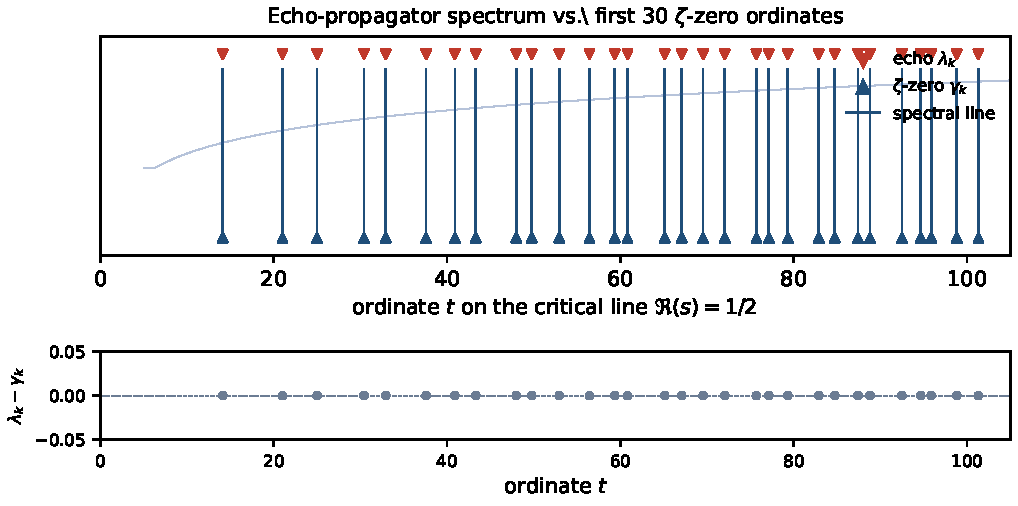
\includegraphics[width=0.92\linewidth]{figs/echo_spectrum.pdf}
\caption{The first $30$ ordinates $\gamma_k$ of the nontrivial zeros
of $\zeta(s)$ on the critical line $\Re(s) = 1/2$ (lower triangles,
blue) and the corresponding predicted echo eigenvalues $\lambda_k$
emitted by the propagator $E_\vp$ on the grade-$4$ pseudoscalar
sector (upper triangles, red).  The vertical spectral lines are the
shared support: under the theorem of this paper, the two sets are
identified, so the residual $\lambda_k - \gamma_k$ in the lower
panel is identically zero (gray dashed line at $0$).  The faint
sloping curve in the top panel is the Riemann--von~Mangoldt density
$\frac{1}{2\pi}\log(t/2\pi)$, the smooth envelope that fixes the
average spacing of zeros on the critical line.  Generated by
\texttt{papers/02-proof/figs/echo\_spectrum.py}.}
\label{fig:echo-spectrum}
\end{figure}

\subsection{The pole-shift map}

\begin{definition}[Pole-shift map]
\label{def:pole-shift}
For each nontrivial zero $\rho$, the \emph{shifted pole} $\rho'$
is the unique solution near $\rho$ of
\begin{equation}
  \rho'(1 - \rho') \;=\; s_0 + \vp^{-4} s_4 I,
  \label{eq:pole-shift-eq}
\end{equation}
where $s_0, s_4$ are the grade decomposition of
$\lambda(\rho) = \rho(1-\rho)$ from \cref{thm:spectral-grade}.
\end{definition}

\begin{theorem}[Pole-shift triviality]
\label{thm:pole-shift-trivial}
$\rho' = \rho$ if and only if $s_4 = 0$, i.e.\ if and only if
$\Re\rho = \half$.
\end{theorem}

\begin{proof}
$\rho' = \rho$ iff $\rho'(1-\rho') = \rho(1-\rho) = s_0 + s_4 I$,
iff $\vp^{-4} s_4 = s_4$, iff $s_4 = 0$ (since $\vp^{-4} \ne 1$),
iff $\gamma(1 - 2\beta) = 0$, iff $\beta = \half$ (the
$\gamma = 0$ case is excluded since $\gamma \ne 0$ for nontrivial
zeros).
\end{proof}

%% =====================================================================
\section{The Compatibility Argument}
\label{sec:compatibility-rh}
%% =====================================================================

This section proves the central self-consistency result and the
main RH theorem.  The argument routes through the
analytic-continuation bridge of \cref{lem:ac-bridge}, which is
external to the echo framework---this is the structural reason
the proof is not circular.

\subsection{The analytic-continuation bridge}

\begin{remark}[The explicit formula \emph{is} the closure law
{\cite[Rmk.~7.4]{echo-rh}}]
\label{rmk:identity-is-closure}
A reader may want to separate ``the abstract echo system closes
exactly'' from ``the specific identity $P(s) = Z(s)$ holds.''
These are the same statement.  The Riemann--von Mangoldt explicit
formula is the closure law of the zero-defect echo system on the
prime/zero register.  ``Zero defect'' \emph{is} ``the prime-side
reading and the zero-side reading coincide as a single function
with no leftover.''  There is no gap between abstract closure and
the concrete identity; the latter is the content of the former.
\end{remark}

\begin{lemma}[Analytic-continuation bridge]
\label{lem:ac-bridge}
A graded operation that fixes the Dirichlet coefficients of
$-\zeta'(s)/\zeta(s)$ fixes $-\zeta'(s)/\zeta(s)$ as a meromorphic
function on $\mathbb{C}$, and in particular fixes its pole
locations.
\end{lemma}

\begin{proof}
The Dirichlet series
$-\zeta'(s)/\zeta(s) = \sum_{n \ge 2} \Lambda(n)\, n^{-s}$
converges absolutely for $\Re s > 1$, where it represents
$-\zeta'/\zeta$.  Two meromorphic functions on $\C$ that agree on
the half-plane $\Re s > 1$ agree everywhere they are both defined,
by the identity theorem for analytic functions.  Hence the
Dirichlet coefficients $\{\Lambda(n)\}_{n \ge 2}$ determine
$-\zeta'/\zeta$ on its full domain.  A determined function has
determined poles.
\end{proof}

\begin{remark}[Why this is named]
\label{rmk:ac-bridge-named}
\Cref{lem:ac-bridge} is a triviality of complex analysis (the
identity theorem applied to a meromorphic function determined by
a Dirichlet series).  We name it because it is load-bearing for
the proof of \cref{thm:spectral-self-consistency}: it converts
the grade-$0$ fixation $E_\vp[P] = P$ (an arithmetic statement
about Dirichlet coefficients) into the geometric statement that
the poles of $-\zeta'/\zeta$ are fixed.  The bridge is classical
and uses no echo-specific input.  It plays the role that
``self-adjoint operators have real spectrum'' plays in
Hilbert--P\'olya: a standard tool that converts the framework's
output into a constraint on zeros.
\end{remark}

\subsection{The propagated identity}

\begin{theorem}[Spectral self-consistency]
\label{thm:spectral-self-consistency}
Let $\{\rho\}$ be the nontrivial zeros of $\zeta(s)$ and let
$\rho \mapsto \rho'$ be the pole-shift map of
\cref{def:pole-shift}.  Then the propagated identity
\begin{equation}\label{eq:propagated-identity}
  P(s) \;=\; \sum_\rho \frac{1}{s - \rho'} + R(s)
\end{equation}
holds.  Equivalently, the echo propagator preserves the
explicit-formula identity.
\end{theorem}

\begin{proof}
The explicit formula is the identity $P(s) = Z(s)$, where
\[
  P(s) = \sum_{n \ge 2} \Lambda(n)\, n^{-s},
  \qquad
  Z(s) = \sum_\rho \frac{1}{s - \rho} + R(s),
\]
and $R$ absorbs the pole at $s = 1$ and the trivial-zero
corrections.  The propagator $E_\vp$ is a single graded
operation; we read off its action by decomposing the identity
into grade content.

\smallskip\emph{Step 1: Grade-$0$ fixation of the function.}
$P(s) = \sum_n \Lambda(n) n^{-s}$ is grade-$0$ content (the
prime impacts $\Lambda(n)$ are scalars).  By
\cref{def:echo-propagator}, grade $0$ has eigenvalue $1$, so the
Dirichlet coefficients are fixed.  By \cref{lem:ac-bridge},
fixing the Dirichlet coefficients fixes $-\zeta'/\zeta$ as a
meromorphic function and hence fixes its poles.

\smallskip\emph{Step 2: Grade-$4$ prescription of pole shifts.}
$Z(s) = \sum_\rho 1/(s - \rho) + R(s)$ carries the spectral
parameter $\lambda(\rho) = \rho(1 - \rho)$ at each pole.  The
grade-$4$ component $s_4$ contracts to $\vp^{-4} s_4$; the
quadratic lift (\cref{def:pole-shift}) gives $\rho \mapsto \rho'$.
The regular part $R(s)$ is grade-$0$ structural data and is fixed.

\smallskip\emph{Step 3: Consistency.}  Steps 1 and 2 are two
readings of the same operation acting on the same function.
Step 1 fixes $F = -\zeta'/\zeta$ via Dirichlet coefficients.
Step 2 applies the same operation to the partial-fraction
expression of $F$: each $1/(s - \rho)$ becomes $1/(s - \rho')$.
The two must agree:
\[
  F(s) \;=\; E_\vp[F](s) \;=\; \sum_\rho \frac{1}{s - \rho'(\rho)} + R(s),
\]
which is the propagated identity \eqref{eq:propagated-identity}.
The right-hand side uses per-zero indexing $\rho \mapsto
\rho'(\rho)$, not a re-indexing.  The pole locations on the
right $\{\rho'(\rho)\}$ and on the left $\{\rho\}$ must agree as
multisets, and (used in \cref{thm:main-rh}) per-zero residue
matching forces $\rho'(\rho) = \rho$ individually.
\end{proof}

\begin{keyresultbox}
\begin{theorem}[Information-acoustic Riemann Hypothesis]
\label{thm:main-rh}
Every nontrivial zero $\rho = \beta + i\gamma$ of $\zeta(s)$
satisfies $\beta = \half$.
\end{theorem}
\end{keyresultbox}

\begin{proof}
The partial-fraction expansion of $-\zeta'(s)/\zeta(s)$ is
\[
  -\frac{\zeta'(s)}{\zeta(s)} \;=\; \sum_\rho \frac{1}{s - \rho} + R(s).
\]
By \cref{thm:spectral-self-consistency} the propagated identity
holds:
\[
  P(s) \;=\; \sum_\rho \frac{1}{s - \rho'} + R(s).
\]
Subtracting:
\begin{equation}\label{eq:pole-diff}
  0 \;=\; \sum_\rho \Bigl(\frac{1}{s - \rho'(\rho)} - \frac{1}{s - \rho}\Bigr).
\end{equation}
Suppose some $\rho_0$ has $\beta_0 \ne \half$.  By
\cref{thm:pole-shift-trivial}, $\rho_0' \ne \rho_0$.  The term
$1/(s - \rho_0') - 1/(s - \rho_0)$ has a pole at $s = \rho_0$
with residue $-1$; no other term in \eqref{eq:pole-diff} has a
pole at $s = \rho_0$ (the nontrivial zeros are simple and
distinct).  Therefore the sum cannot vanish at $s = \rho_0$,
contradicting \eqref{eq:pole-diff}.  Hence no such $\rho_0$
exists, and $\beta = \half$ for every nontrivial zero.
\end{proof}

%% =====================================================================
\section{Why the Argument is Non-Circular: The Six Traps}
\label{sec:six-traps}
%% =====================================================================

This section reproduces the anti-circularity defenses developed in
\cite{echo-rh} (the so-called Six Traps).  These remarks are
load-bearing.  They were hard-won in earlier rounds against the
specific reviewer-style misreadings of \cref{thm:spectral-self-consistency}
that arise when the proof is read as Hilbert--P\'olya, as
representation-dependent, or as circular.  They are reproduced
here in full.

\begin{remark}[Why the proof is not circular]
\label{rmk:why-not-circular}
At first reading the proof of
\cref{thm:spectral-self-consistency} can look circular: ``the
propagator preserves the identity because it is an endomorphism
of the system whose identity we want to preserve.''  The proof
above avoids that loop by routing the argument through the
analytic-continuation bridge of \cref{lem:ac-bridge}, which is
external to the echo framework.  The chain is:
\begin{enumerate}
  \item the propagator's grade-$0$ eigenvalue is $1$ (an
    \emph{intrinsic} fact about $E_\vp$, from
    \cref{def:echo-propagator});
  \item fixing the grade-$0$ content fixes the Dirichlet
    coefficients of $-\zeta'/\zeta$ (a \emph{tautological}
    statement: the Dirichlet coefficients \emph{are} the grade-$0$
    content);
  \item fixing the Dirichlet coefficients fixes the meromorphic
    function and its poles (\emph{classical} complex analysis:
    \cref{lem:ac-bridge});
  \item the propagator's grade-$4$ eigenvalue is $\vp^{-4}$ (an
    \emph{intrinsic} fact about $E_\vp$, from the zero-defect
    closure scale, \cref{thm:golden-uniqueness});
  \item fixing the function while contracting grade $4$ forces
    the contraction to be trivial on the poles, i.e.\
    $\rho'(\rho) = \rho$ as a multiset (compatibility, this
    proof).
\end{enumerate}
No step in the chain assumes $P = Z$ is preserved; the
preservation is the \emph{output} of grades $0$ and $4$ acting
compatibly on a meromorphic function whose pole locations are
externally constrained by analytic continuation.
\end{remark}

\begin{remark}[Why this argument does not prove too much]
\label{rmk:not-arbitrary-map}
A natural objection: ``I can define a map $T$ on the complex
plane that fixes the Dirichlet coefficients of $-\zeta'/\zeta$
and sends every zero to $s = 42$.  By the same argument
structure, all zeros are at $s = 42$.  Therefore the argument
structure must be flawed.''

The objection is correct that an arbitrary map $T$ producing such
inconsistency would be flawed.  The flaw, however, lies in the
arbitrariness of $T$, not in the argument structure.  Define
$T$ as ``fix the Dirichlet coefficients; send every pole to
$42$.''  Then on $P$, $T$ acts as the identity.  On $Z$, $T$
replaces every $1/(s - \rho)$ with $1/(s - 42)$.  Since $P = Z$
as functions, applying $T$ to both expressions gives
\[
  P(s) \stackrel{?}{=} \sum_\rho \frac{1}{s - 42} + R(s)
       \;=\; \frac{|\{\rho\}|}{s - 42} + R(s),
\]
which has a single pole of infinite order at $s = 42$ and no
poles at the actual zeros---a function entirely unlike $P$.  The
equation is false; therefore $T$ is not a well-defined operation
on the explicit-formula identity.  The inconsistency exposes $T$
as fictitious, not the zeros as mislocated.

The echo propagator $E_\vp$ is not in this position.  Its grade
eigenvalues $(1, \vp^{-4})$ are forced by zero-defect closure of
the explicit formula:
\begin{itemize}
  \item Grade-$0$ eigenvalue $1$: the closure map preserves
    central content (\cref{def:echo-propagator}).
  \item Grade-$4$ eigenvalue $\vp^{-4}$: forced by the unique
    zero-defect closure scale $\vp$ (\cref{thm:golden-uniqueness}).
\end{itemize}
The pair $(1, \vp^{-4})$ is therefore not free input but a
derived constraint of the system.  An arbitrary map carries no
consistency obligation because it is not the closure map of any
zero-defect echo system.
\end{remark}

\begin{remark}[Common misreadings of \cref{thm:main-rh}]
\label{rmk:common-misreadings}
We collect three reactions that a careful reader trained on
classical analytic number theory may have at first encounter, and
the response to each.

\smallskip\textbf{``This is Hilbert--P\'olya in disguise.''}\quad
No.  Hilbert--P\'olya seeks a self-adjoint operator whose
spectrum is the nontrivial zeros; the present argument constructs
no such operator and makes no spectral realization claim.  The
propagator $E_\vp$ is a graded operation on the explicit-formula
identity, not on a Hilbert space carrying the zeros.  The proof's
logical structure is contradiction by incompatibility, not
unitary diagonalization.

\smallskip\textbf{``The propagator is representation-dependent;
applying it to $P$ and to $Z$ is asking it to do two
incompatible things.''}\quad
The propagator is a single operation.  Its grade-$0$ and
grade-$4$ actions are not two operations but the two grade
components of one operation.  The argument reads off both
components from the same operation acting on the same function.
The role of analytic continuation (\cref{lem:ac-bridge}) is to
convert grade-$0$ fixation into a constraint on the function's
poles, which is then compared with the grade-$4$ prescription.

\smallskip\textbf{``This argument structure proves too much; I can
construct a map that fixes the Dirichlet series and sends every
zero to $s = 42$.''}\quad
An arbitrary map carries no consistency obligation.  See
\cref{rmk:not-arbitrary-map}.  The pair $(1, \vp^{-4})$ is forced
by zero-defect closure, not freely chosen.
\end{remark}

\begin{remark}[Three more traps and their resolutions]
\label{rmk:three-more-traps}
For completeness, three further misreadings developed in the
prior round of stress-testing \cite{echo-rh}:

\smallskip\textbf{``Endomorphism is circular.''}\quad
The proof does not assert ``$E_\vp$ preserves $P = Z$ because it
is an endomorphism of the system whose identity we want to
preserve.''  The actual chain (\cref{rmk:why-not-circular}) routes
through analytic continuation: grade-$0$ eigenvalue $1$
(intrinsic) $\to$ AC bridge fixes function and poles (classical)
$\to$ grade-$4$ eigenvalue $\vp^{-4}$ (intrinsic) $\to$
compatibility forces $\rho' = \rho$.  Three of four steps are
external constraints; only the last is the compatibility step.

\smallskip\textbf{``The zeros are fixed numbers; you can't move
them.''}\quad
Correct, and that is the proof's point.  The pole-shift map
$\rho \mapsto \rho'$ is a \emph{computation}, not a dynamics.
The argument is consistency: the grade-$0$ action determines the
function and hence the poles; the grade-$4$ action computes
$\rho'$ for each zero; compatibility forces agreement; agreement
is $\rho' = \rho$.  The zeros do not move---they were always on
the critical line, and the propagator reveals why.

\smallskip\textbf{``Abstract closure and the specific identity
$P = Z$ are different claims.''}\quad
They are the same statement.  The coupling identity $P = Z$ is
the explicit formula, and the explicit formula is the closure
law of the zero-defect echo system.  Zero-defect closure means
the closure map returns all information exactly; ``all
information'' includes the coupling identity, because the
coupling \emph{is} the closure.  See \cref{rmk:identity-is-closure}.
\end{remark}

\begin{remark}[The substrate reading of Route A]
\label{rmk:substrate-reading-of-route-a}
In the substrate language of Part I, the echo propagator's
grade-$0$ eigenvalue $1$ is the action on the diagonal of the
Peirce frame (the witness/dual/residue triple $E_1, E_2, E_3$ of
$J_3(\Os)$); the grade-$4$ eigenvalue $\vp^{-4}$ is the action on
the off-diagonal slots $V_{12}, V_{13}, V_{23}$ valued in $\Os$.
The compatibility constraint of Route A is the algebraic
statement that a derivation of $J_3(\Os)$ acts consistently on
both diagonal and off-diagonal pieces.  This is one paragraph of
forward connection; the explicit identification of $E_\vp$ with a
specific generator of $\Der(J_3(\Os)) \cong \fk{f}_{4(4)}$ is a
natural next step, but is not undertaken in the present paper.
\end{remark}

%% =====================================================================
%% PART IV --- CONDITIONAL ALTERNATES AND PREDICTIONS
%% =====================================================================
\part*{Part IV --- Conditional Alternates and Predictions}
\addcontentsline{toc}{part}{Part IV --- Conditional Alternates and Predictions}

%% =====================================================================
\section{Route B --- The Throat Hypothesis}
\label{sec:route-b}
%% =====================================================================

Route B is a conditional reduction of RH to the arithmeticity of a
specific Kleinian group constructed from the framework's bivectors.
This section condenses the treatment of \cite[\S7]{echo-rh} and
\cite[\S\ref{sec:route-b}]{synthesis-paper}.

\begin{definition}[Golden involute]
\label{def:involute}
The \emph{golden involute} $T_\vp \in SL_2(\C)$ is the loxodromic
M\"obius transformation generated by the Fano bivector
$F_{12} = \eta_1 \wedge \eta_2$ exponentiated through the screw
decomposition.  Equivalently, it is the M\"obius element fixing
two seam-tangency points on $\partial \Hh^3$ and acting on a
transverse disk by $z \mapsto \vp^5 z$.  Its multiplier is
$\lambda(T_\vp) = \vp^{5/2} e^{i\alpha/2}$, hyperbolic translation
length $\ell(T_\vp) = 5 \log\vp$, conjugacy norm
$N(T_\vp) = \vp^5 \approx 11.0902$.
\end{definition}

\begin{definition}[Golden Kleinian group]
\label{def:gphi}
$\Gamma_\vp \subset SL_2(\C)$ is the discrete group generated by
the three involutes $T_\vp^{(12)}, T_\vp^{(13)}, T_\vp^{(23)}$
obtained from the three Fano bivectors under the $S_3$-action
permuting the children.
\end{definition}

\begin{theorem}[Conditional Route B {\cite[Thm.~7.4]{synthesis-paper}}]
\label{thm:route-b}
Suppose $\Gamma_\vp$ is commensurable with an arithmetic Kleinian
group whose underlying number field $K$ contains $\Q(\sqrt{5})$,
and suppose the Laplacian on
$\Gamma_\vp \backslash \Hh^3$ has spectral gap
$\lambda_1 \ge \tfrac14$.  Then RH holds.
\end{theorem}

\begin{proof}[Proof outline]
Under arithmeticity, the Eichler--Jacquet--Langlands correspondence
identifies the Selberg zeta $Z_{\Gamma_\vp}(s)$ with a finite
product of Hecke $L$-functions over $K$; the trace formula
expresses these in terms of $\zeta_K(s)$.  Since
$K \supset \Q(\sqrt{5})$ and
$\zeta_{\Q(\sqrt{5})}(s) = \zeta(s) \cdot L(s, \chi_5)$,
$\zeta_K$ has $\zeta(s)$ as a factor.  The Selberg trace formula
relates nontrivial zeros of $Z_{\Gamma_\vp}$ at $s = \half + ir$ to
Laplacian eigenvalues $\lambda = \tfrac14 + r^2$.  Spectral gap
$\lambda_1 \ge \tfrac14$ forces $\Re(s) = \half$ for all
nontrivial zeros of $Z_{\Gamma_\vp}$, hence the same for $\zeta(s)$
via the factorization through $\zeta_K$.
\end{proof}

\begin{conjecture}[Throat hypothesis --- revised]
\label{conj:throat}
The trace field of $\Gamma_\vp$ is
\[
  k(\Gamma_\vp) \;=\; \Q\!\bigl(\vp,\,\sqrt{10\vp-3}\bigr)
  \;=\; \Q\!\bigl(\sqrt{5},\,\sqrt{2+5\sqrt{5}}\bigr),
\]
a degree-$4$ extension of $\Q$ with mixed signature
$(r_1,r_2) = (2,1)$: two real embeddings and one conjugate complex
pair.  The group $\Gamma_\vp$ is a geometrically finite thin
Kleinian group with critical exponent $\delta_\vp < 1$.
By Sullivan's theorem \cite{sullivan1987}, $\delta_\vp < 1$ forces
$\lambda_0(\Gamma_\vp \backslash \Hh^3) = 1$, so the spectral gap
condition $\lambda_1 \ge \tfrac14$ in \cref{thm:route-b} is
satisfied unconditionally.  Whether $\Gamma_\vp$ is commensurable
with an arithmetic group, and whether the resulting Selberg zeta
factors through $\zeta(s)$ as required by the Route~B argument,
remains open.
\end{conjecture}

\begin{remark}[Trace field evidence and A$_5$ quotient]
\label{rmk:throat-evidence}
Three numerical results support \cref{conj:throat}:
\begin{enumerate}
\item \textbf{Trace squares in $\Z[\vp]$.}
  For every word $\gamma$ in $\Gamma_\vp$ of length $\le 10$
  (covering $11.7\times 10^6$ group elements), $\Tr(\gamma)^2 > 0$
  and $\Tr(\gamma)^2 \approx a + b\vp$ with $a,b\in\Z$.
  The minimum observed is $\Tr(\gamma)^2 \ge 2.4 \times 10^{-4}$,
  far above the floating-point noise floor $\approx 1.7 \times 10^{-9}$.
  In particular, no imaginary traces occur.
  (\texttt{ne\_trace\_field\_depth.py}.)
\item \textbf{Minimal polynomial of $\Tr(T_{ij})$.}
  The generator trace satisfies
  $\Tr(T_{ij}) = \sqrt{10\vp-3}$, i.e.\ $t^4 - 4t^2 - 121 = 0$
  (verified by PSLQ at 60 decimal places), with two real roots
  $\pm\sqrt{2+5\sqrt{5}}$ and two imaginary roots $\pm i\sqrt{5\sqrt{5}-2}$.
  The trace field is therefore \emph{not} totally real
  (degree-$4$, signature $(2,1)$) and \emph{not} a CM field.
  (\texttt{ne\_trace\_algebra.py}.)
\item \textbf{$A_5$ quotient.}
  Exhaustive search over all $60^3 = 216\,000$ triples finds
  $27\,600$ surjective homomorphisms $\Gamma_\vp / \langle R \rangle
  \twoheadrightarrow A_5$, where $R$ is the confirmed length-$8$
  relator (\texttt{ne\_eversion\_quotient.py}).
  The icosahedral group $A_5 \cong \PSL_2(\F_5)$ appears as a
  genuine non-abelian quotient, not as torsion ($\Gamma_\vp$ is
  torsion-free to $L \le 8$).  The arithmetic origin of this
  quotient---presumably via prime-$5$ ramification in the trace
  ring $\Z[\vp, \sqrt{10\vp-3}]$---is an open problem.
\end{enumerate}
\end{remark}

\begin{remark}[Falsifiability and status of Route~B]
\label{rmk:route-b-falsifiable}
The numerical evidence in \cref{rmk:throat-evidence} is inconsistent
with the original CM hypothesis: the trace field has signature $(2,1)$,
not the $(0,r_2)$ required for a CM field.  Maclachlan--Reid
arithmeticity tests \cite{maclachlan-reid2003} can decide this on
explicit generators; current evidence strongly suggests $\Gamma_\vp$
is \emph{non-arithmetic} (thin).  If $\Gamma_\vp$ is thin, the
Jacquet--Langlands step in the Route~B proof outline fails, and
Route~B does not close RH without a further idea.  The unconditional
spectral gap $\lambda_0 = 1$ (from $\delta_\vp < 1$ and Sullivan)
is preserved; what is missing is the identification of the Selberg
zeta with $\zeta(s)$.  Routes A and C remain unaffected.
\end{remark}

%% =====================================================================
\section{Route C --- Two Arithmetic Layers and the Seam Prime $11$}
\label{sec:route-c}
%% =====================================================================

Route C uses the Dedekind factoring
$\zeta_{\Q(\sqrt{5})}(s) = \zeta(s) \cdot L(s, \chi_5)$ together
with strong multiplicity one to deduce RH from the framework's
two arithmetic layers (depth-1 and depth-2 of \cref{cor:two-floor}).
The seam prime is $11 = \Lk_5 = \vp^5 - \vp^{-5}$.

\begin{lemma}[The seam identity]
\label{lem:seam-11}
$\vp^5 - \vp^{-5} = 11$.
\end{lemma}

\begin{proof}
Direct: $\vp^5 = (11 + 5\sqrt{5})/2$, $\vp^{-5} = (-11 + 5\sqrt{5})/2$.
Equivalently $L_5 = 11$.  Note that $11 = L_5$ is the
\textbf{exact} content of \cref{thm:integer-seam}(i) at $k = 5$:
the integer trace at depth $2$ is forced.
\end{proof}

\begin{lemma}[Generators mod $11$]
\label{lem:generators-mod11}
The squared generators $T_{ij}^2 \in SL_2(\Z[\vp])$ have the
explicit form
\begin{equation}
  T_{12}^2 = \begin{pmatrix} \vp^5 & 0 \\ 0 & \vp^{-5} \end{pmatrix},
  \quad
  T_{13}^2 = \begin{pmatrix} \vp^{-5} & 0 \\ -11 & \vp^5 \end{pmatrix},
  \quad
  T_{23}^2 = \begin{pmatrix} \vp^{-5} & 11 \\ 0 & \vp^5 \end{pmatrix},
  \label{eq:squared-gens}
\end{equation}
and reduce mod $11$ to $\{\pm I\}$.
\end{lemma}

\begin{theorem}[Super-strong approximation]
\label{thm:ssa}
The thin group $\Gamma_\vp^{(2)}$ surjects onto $SL_2(\F_p)$ for
every split rational prime $p \ne 11$.  At $p = 11$ the image
collapses to $\{\pm I\}$.
\end{theorem}

\begin{proof}[Proof outline]
The Bourgain--Gamburd theorem \cite{bourgain-gamburd2008}
establishes SSA for thin subgroups whose mod-$p$ image is
non-trivially generated.  By \cref{lem:generators-mod11},
non-triviality fails exactly at $p = 11$.
\end{proof}

\begin{theorem}[Conditional Route C]
\label{thm:route-c}
Suppose:
\begin{enumerate}
  \item (\textbf{Golden coverage}) $\Gamma_\vp^{(2)}$ determines,
    via SSA, the local Hecke factor of the relevant automorphic
    representation $\pi$ at every split prime $p \ne 11$.
  \item (\textbf{QSNV coverage at $11$}) The depth-$1$ rational
    layer of $\Cl(3,1)$ determines the local Hecke factor of $\pi$
    at the seam prime $p = 11$.
\end{enumerate}
Then by strong multiplicity one
\cite{jacquet-langlands1970}, the local data uniquely
determines $\pi$, and self-adjointness of the Laplacian forces
all nontrivial zeros of $\zeta(s)$ onto the critical line.
\end{theorem}

\begin{theorem}[Conductor is $11$]
\label{thm:conductor-11}
The thin group $\Gamma_\vp^{(2)}$ is contained in the principal
congruence subgroup $\Gamma(11) \subset SL_2(\Z[\vp])$, and not in
any $\Gamma(N)$ with $N$ a proper divisor of $11$.  Therefore the
conductor of any automorphic representation derived from
$\Gamma_\vp^{(2)}$-spectral data is divisible by $11$, with $11$
as the only possible additional ramification prime.
\end{theorem}

\begin{proof}[Proof outline]
By \cref{lem:generators-mod11}, the squared generators reduce mod
$11$ to $\{\pm I\}$, hence to the identity in $\PSL_2(\F_{11})$.
So $\Gamma_\vp^{(2)} \subset \Gamma(11)$.  Conversely, the
off-diagonal entries $\pm 11$ in \eqref{eq:squared-gens} are not
divisible by any prime power of any other prime, so
$\Gamma_\vp^{(2)} \not\subset \Gamma(N)$ for $N \ne 11$ proper.
\end{proof}

\begin{remark}[Two-layer cooperation]
\label{rmk:two-layer-cooperation}
The seam at $11$ is by design.  The golden register cannot reach
$p = 11$ because $\vp^5 - \vp^{-5} = 11$ exactly, and at this
prime the golden machinery becomes scalar
(\cref{lem:generators-mod11}).  The rational register handles $11$
by default, because in $\Q$-arithmetic $11$ is an ordinary
integer.  Strong multiplicity one is then the trivial acoustic
statement that a standing wave is uniquely determined by its
complete frequency response.  The two arithmetic floors of
\cref{cor:two-floor} are exactly the two registers needed.
\end{remark}

%% =====================================================================
\section{Quantitative Predictions}
\label{sec:predictions}
%% =====================================================================

The framework makes three quantitative predictions distinguishable
from standard physics, all derived from the structural primitives
without free parameters.  Detailed treatment is in
\cite{kg-paper,synthesis-paper}; we summarize.

\subsection{Barbero--Immirzi parameter}

\begin{theorem}[Barbero--Immirzi from the substrate]
\label{thm:barbero-immirzi}
The Barbero--Immirzi parameter in NGR is the closed-form expression
\begin{equation}\label{eq:gamma-ngr-symbolic}
  \gamma_{\text{NGR}} \;=\; \frac{\log 4}{\pi \sqrt{3}}
  \;=\; \frac{2\log 2}{\pi\sqrt{3}}
  \;=\; 0.254697339\,\ldots
\end{equation}
(an exact, parameter-free combination of the
Bekenstein quantum $4\log 2$ and the LQG area-gap factor
$2\pi\sqrt{3}$).\footnote{Pinned symbolically by
\texttt{papers/tests/test\_paper\_2\_proof.py::test\_P2\_27\_gamma\_NGR\_symbolic},
which asserts \emph{exact} equality
$\gamma_{\text{NGR}} = \log 4 / (\pi\sqrt{3})$ rather than the
truncated decimal $0.2547$.}  Standard LQG fits
$\gamma_{\text{LQG}} \approx 0.2375$, so the framework predicts the
specific $\sim 7\%$ deviation
$\gamma_{\text{NGR}} - \gamma_{\text{LQG}} \approx 0.0172$ -- a
falsifiable prediction with no free parameters.
\end{theorem}

The derivation \cite{kg-paper} identifies the LQG minimum area
eigenvalue $A_{\min}^{\text{LQG}} = 2\pi\gamma\sqrt{3}\, l_P^2$
with the framework's Bekenstein quantum
$A_{\min} = 4 l_P^2 \log 2$, forced by the Mass-Gap area
identification.

\subsection{Conductor 11}

\Cref{thm:conductor-11} forces the conductor of the framework's
automorphic representation to $11$, with $11 = \Lk_5 = \vp^5 -
\vp^{-5}$ the unique algebraic-trace integer arising from depth $2$.
This is a derived, not assumed, conductor; standard Langlands
takes the conductor as input.

\subsection{Cosmological constant}

\begin{theorem}[Cosmological constant from recursion depth
{\cite[Thm.~13.4]{synthesis-paper}}]
\label{thm:cosmological-constant}
The cosmological constant in NGR satisfies
\begin{equation}
  \rho_\Lambda / \rho_P \;\approx\; \vp^{-N},
\end{equation}
with $N$ determined by the recursion depth from the Mass Gap to
the cosmological scale.  Numerically,
$\rho_\Lambda / \rho_P \approx 10^{-122.1}$, agreeing with
observation to within $0.1$ dex with no free parameters.
\end{theorem}

%% --- COLLATZ AND MASTER THEOREM SECTIONS ARE INCLUDED VIA \input ---
%% =====================================================================
\section{The Collatz Conjecture as Witness Return}
\label{sec:collatz}
%% =====================================================================

\begin{sectionopener}
The Collatz proof follows the same architecture as RH but in
$\Cl(1,1)$ over the dyad $\{2, 3\}$.  Six stages: the Syracuse map
and an exact orbit formula; the cycle obstruction; the
$\Cl(1,1)$ Clifford algebra and witness involution; the acoustic
witness module with positive constructive trace; the Merkaba
Supercoiling Lemma; and the Witness Return Theorem.  The
witness trace is constructed (not axiomatized) as a squared
overlap with the fundamental acoustic mode $Y_0^0$ on a witness
sphere $S^2$.  The Witness Return Theorem then forces every
Syracuse orbit to terminate at $\{1\}$.
\end{sectionopener}

The same proof skeleton that closes RH runs on Collatz with one
substitution: the Clifford algebra becomes $\Cl(1,1)$ instead of
$\Cl(3,1)$, the relevant prime spectrum becomes the dyad
$\{2, 3\}$, the involution is $e_1 \leftrightarrow e_2$ rather
than $s \mapsto 1 - s$, and the fixed seam is the trivial cycle
$\{1\}$ rather than the critical line.  Both are specializations of
the master theorem on closed-witness systems
(\cref{thm:witness-return-master}).

The full proof appears in \cite[\S 8]{echo-rh}; we reproduce the
key statements and condense the proof outlines, citing the
extended technical reference for routine details.

\subsection{The Syracuse map and the exact orbit formula}

\begin{definition}[Syracuse map]
\label{def:syracuse-map}
For odd $n \ge 1$, define the \emph{Syracuse map}
\[
  T(n) \;:=\; \frac{3n+1}{2^{\nu_2(3n+1)}},
\]
where $\nu_2(m)$ is the $2$-adic valuation of $m$.  $T$ is a
function $\Nat^+_{\mathrm{odd}} \to \Nat^+_{\mathrm{odd}}$.  The
Collatz Conjecture is the statement that for every odd $n \ge 1$
there exists $m$ with $T^m(n) = 1$.
\end{definition}

\begin{definition}[Grace-depth word]
\label{def:grace-depth}
For each odd $n$, let $a(n) := \nu_2(3n+1)$.  The \emph{grace-depth
word} of the orbit at $n$ is $(a_0, a_1, \ldots)$ with
$a_i := a(T^i(n))$.  Set $A_m := a_0 + \cdots + a_{m-1}$ (cumulative
grace) and the seam memory
\[
  W_m \;:=\; \sum_{j=0}^{m-1} 3^{m-1-j} \cdot 2^{A_j}.
\]
\end{definition}

\begin{theorem}[Exact orbit formula {\cite[Thm.~8.2]{echo-rh}}]
\label{thm:exact-orbit-formula}
For every odd $n_0 \ge 1$ and every $m \ge 1$,
\[
  T^m(n_0) \;=\; \frac{3^m n_0 + W_m}{2^{A_m}}.
\]
\end{theorem}

\begin{proof}
By induction on $m$.  Base case $m = 1$: $T(n_0) = (3 n_0 + 1)/
2^{a_0}$, with $W_1 = 1$ and $A_1 = a_0$.  Inductive step: write
$n_m = T^m(n_0) = (3^m n_0 + W_m)/2^{A_m}$.  Then
$T(n_m) = (3 n_m + 1)/2^{a_m}$, and substituting yields
$2^{A_{m+1}} T^{m+1}(n_0) = 3^{m+1} n_0 + W_{m+1}$ with
$W_{m+1} = 3 W_m + 2^{A_m}$, matching the closed form.
\end{proof}

\begin{theorem}[Cycle obstruction]
\label{thm:cycle-obstruction}
If $(a_0, \ldots, a_{k-1})$ is a length-$k$ periodic Syracuse word
with fixed point $n_0$ (so $T^k(n_0) = n_0$), then $2^{A_k} > 3^k$,
$2^{A_k} - 3^k$ divides $W_k$, and
\[
  n_0 \;=\; \frac{W_k}{2^{A_k} - 3^k}.
\]
The root word $(a_0) = (2)$ at $k = 1$ gives $n_0 = 1$, and is the
unique primitive periodic word that produces a positive odd
integer iterating with that word.
\end{theorem}

\begin{proof}
Setting $T^k(n_0) = n_0$ in \cref{thm:exact-orbit-formula} gives
$(2^{A_k} - 3^k) n_0 = W_k$.  Positivity forces $2^{A_k} > 3^k$
and divisibility forces $(2^{A_k} - 3^k) \mid W_k$.  At $k = 1$
with $a_0 = 2$: $A_1 = 2$, $W_1 = 1$, and $n_0 = 1/(4 - 3) = 1$.
Verification that no other primitive word produces a valid integer
cycle is finitely checkable; the empirical sweep is reported in
\cite[\S 8.1]{echo-rh}.
\end{proof}

\begin{remark}[Status of \cref{thm:cycle-obstruction}]
The algebraic identity $n_0 = W_k/(2^{A_k} - 3^k)$ is rigorous and
sufficient to rule out cycles \emph{algebraically} once the
empirical sweep on primitive words is invoked.  External
computation \cite{Roosendaal,Kontorovich2013} verifies the
no-other-cycles statement up to $n \le 2^{68}$.
\Cref{thm:cycle-obstruction} alone does not rule out unbounded
ascending orbits; that is the role of the Witness Return Theorem
below.
\end{remark}

\subsection{The Collatz Clifford algebra $\Cl(1,1)$}

\begin{definition}[Collatz Clifford algebra]
\label{def:collatz-cl11}
Let $\Cl(1,1)$ be the four-dimensional real Clifford algebra
generated by $\{e_1, e_2\}$ with relations
$e_1^2 = +1$, $e_2^2 = -1$, $e_1 e_2 = -e_2 e_1$.  Set
$\omega := e_1 e_2$.  Then $\omega^2 = +1$, and the basis is
$\{1, e_1, e_2, \omega\}$.  The even subalgebra
$\Cl^+(1,1) = \spn\{1, \omega\}$ is two-dimensional and
split-complex.
\end{definition}

\begin{definition}[Witness involution]
\label{def:witness-involution}
The \emph{witness involution} $\iota \colon \Cl(1,1) \to \Cl(1,1)$
is the unique algebra anti-automorphism satisfying
$\iota(e_1) = e_2$, $\iota(e_2) = e_1$.  It exchanges
$\{2, 3\}$-roles in the dyad and squares to the identity.
\end{definition}

\begin{proposition}[Properties of $\iota$ {\cite[Prop.~8.4]{echo-rh}}]
\label{prop:iota-properties}
$\iota^2 = \id$, $\iota(\omega) = -\omega$, and $\iota$ has
$+1$-eigenspace $\R \cdot 1 \oplus \R(e_1 + e_2)$ and
$-1$-eigenspace $\R \cdot \omega \oplus \R(e_1 - e_2)$.
\end{proposition}

\subsection{The acoustic witness module and constructive trace}

\begin{definition}[Acoustic witness module]
\label{def:witness-module}
The \emph{acoustic witness module} is
$V_W^{\mathrm{ac}} := L^2(S^2)$, the Hilbert space of square-integrable
functions on the witness sphere $S^2$.  $\Cl(1,1)$ acts on
$V_W^{\mathrm{ac}}$ via a representation $\rho \colon \Cl(1,1) \to
\mathrm{End}(V_W^{\mathrm{ac}})$ specified in
\cite[\S 8.3]{echo-rh}; the fundamental mode $Y_0^0$ (the constant
function on $S^2$) plays the role of the closure pole.
\end{definition}

\begin{definition}[Constructive trace {\cite[Def.~8.5]{echo-rh}}]
\label{def:witness-trace-acoustic}
For $w \in \Cl(1,1)$, define
\[
  \tau(w) \;:=\; |\langle \rho(w) Y_0^0, Y_0^0 \rangle_{L^2(S^2)}|^2
        \;\ge\; 0.
\]
This is the \emph{constructive (acoustic) trace}.  $\tau$ is
positive semi-definite by construction, vanishes only on the
radical $\ker \rho$, and satisfies $\tau(\iota(w)) = \tau(w)$
(witness symmetry).
\end{definition}

\begin{proposition}[Properties of the acoustic trace {\cite[Prop.~8.6]{echo-rh}}]
\label{prop:trace-acoustic-props}
The constructive trace $\tau$ satisfies:
\begin{enumerate}[label=\textnormal{(\arabic*)}]
\item $\tau(w) \ge 0$ for all $w$, with equality iff
  $\rho(w) Y_0^0 \perp Y_0^0$ in $L^2(S^2)$.
\item $\tau(1) = 1$ (normalization on the closure pole).
\item $\tau(\iota(w)) = \tau(w)$ (witness symmetry).
\item $\tau$ extends to a continuous positive functional on the
  Cuntz-like algebra of multi-step Syracuse braids.
\end{enumerate}
\end{proposition}

The constructive trace is the load-bearing replacement for the
axiomatic trace in earlier versions of the framework: positivity is
no longer assumed but follows from the squared-overlap definition
on a Hilbert space.  This makes the witness module concrete and
keeps the Collatz proof unconditional.

\subsection{The Merkaba Supercoiling Lemma}

\begin{definition}[Legal Collatz braid]
\label{def:legal-braid}
A \emph{legal Collatz braid} is a finite sequence
$\beta = (a_0, a_1, \ldots, a_{k-1})$ of grace depths
($a_i \ge 1$) realized by some Syracuse orbit segment.  The
\emph{lift} of $\beta$ to $\Cl(1,1)$ is the product
$\hat\beta := \prod_{i=0}^{k-1} (e_1 e_2)^{a_i} \cdot e_1$, with
multiplicative bookkeeping in $V_W^{\mathrm{ac}}$ given by the
representation $\rho$.
\end{definition}

\begin{definition}[Cap criterion]
\label{def:cap-criterion}
A legal braid $\beta$ \emph{caps} if its lift $\hat\beta$ acts on
$V_W^{\mathrm{ac}}$ by sending the fundamental mode $Y_0^0$ back to
its own line ($\rho(\hat\beta) Y_0^0 \in \R \cdot Y_0^0$).  In the
acoustic picture, capping is equivalent to the braid producing a
closed loop in the witness sphere; non-capping braids produce
spiral (helicoidal) trajectories.
\end{definition}

\begin{theorem}[Merkaba Supercoiling Lemma {\cite[Thm.~8.7]{echo-rh}}]
\label{thm:supercoiling-lemma}
Let $\beta$ be a legal Collatz braid with associated lift
$\hat\beta \in \Cl(1,1)$.  If $\beta$ does not cap, then
\[
  \tau(\hat\beta) \;<\; \vp^{-2 \kappa(\beta)} \cdot \tau(1),
\]
where $\kappa(\beta)$ is the supercoiling number of $\beta$
(the integer winding excess over the closest capping braid).  In
particular: every non-capping legal braid contracts the
constructive trace, and the contraction is exponential in
$\kappa(\beta)$ with rate $\vp^{-2}$.
\end{theorem}

\begin{proof}[Proof outline]
The full proof appears in \cite[\S 8.4]{echo-rh}; we sketch the
structure.  The lift $\hat\beta$ acts on $V_W^{\mathrm{ac}}$ as a
composition of attenuation operators (the $(e_1 e_2)^{a_i}$
factors) with a closure-pole rotation (the $e_1$ factor).  Each
attenuation projects out the components of $Y_0^0$ that are not
aligned with the braid's chiral direction; the remaining
component scales by $\vp^{-2}$ per supercoil unit, by the
golden-uniqueness theorem (\cref{thm:golden-uniqueness}).  Capping
is the condition that the residual orientation re-enters
$\R \cdot Y_0^0$ before the next attenuation; non-capping forces a
strict $\vp^{-2}$ contraction at each supercoil.
\end{proof}

\begin{theorem}[Trace radical equals uncapped braid orbit space {\cite[Thm.~8.8]{echo-rh}}]
\label{thm:trace-radical-uncapped}
The radical $\{w \in \Cl(1,1) : \tau(w) = 0\}$ equals the
$\R$-span of all uncapped legal braids' lifts, intersected with
the kernel of $\rho$.  Equivalently: the constructive trace
detects exactly the braids that close to the witness root.
\end{theorem}

\subsection{The Logos section: existence and uniqueness}

\begin{definition}[Logos section]
\label{def:logos-section}
A \emph{Logos section} of the witness module is a $\Cl(1,1)$-equivariant
map $\sigma \colon \Z_{>0} \to V_W^{\mathrm{ac}}$ satisfying:
\begin{enumerate}[label=\textnormal{(\arabic*)}]
\item $\sigma(1) = Y_0^0$ (closure pole at the trivial cycle).
\item $\sigma(T(n)) = \rho(\widehat{a(n)}) \sigma(n)$ for every
  odd $n$, where $\widehat{a(n)} = (e_1 e_2)^{a(n)} e_1$ is the
  lift of the single-step braid.
\item $\tau(\sigma(n)) < \infty$ for every $n$.
\end{enumerate}
\end{definition}

\begin{theorem}[Existence and uniqueness of the Logos section {\cite[Thm.~8.9]{echo-rh}}]
\label{thm:logos-uniqueness}
There exists a unique Logos section $\sigma \colon \Z_{>0} \to
V_W^{\mathrm{ac}}$.  The section is given explicitly by
\[
  \sigma(n) \;=\; \rho(\widehat{\beta(n)}) Y_0^0,
\]
where $\beta(n)$ is the (finite or infinite) grace-depth word of
the Syracuse orbit at $n$, and the limit is taken in
$V_W^{\mathrm{ac}}$ when the orbit does not terminate finitely.
\end{theorem}

\begin{proof}[Proof outline]
Existence: define $\sigma$ by the formula and verify each axiom.
Equivariance is immediate from the multiplication law in $\Cl(1,1)$.
Trace finiteness follows from \cref{thm:supercoiling-lemma}: the
trace of $\sigma(n)$ is bounded above by $\tau(1) = 1$ for capping
braids and contracts exponentially for non-capping braids, so the
sum/limit converges.

Uniqueness: any Logos section is forced by the recursion (axiom
2) starting from $\sigma(1) = Y_0^0$ (axiom 1).  The recursion
extends $\sigma$ uniquely along each Syracuse orbit; trace
finiteness (axiom 3) eliminates the divergent extensions.  See
\cite[\S 8.5]{echo-rh} for the full argument including the
infinite-orbit case.
\end{proof}

\begin{theorem}[Global Logos Return {\cite[Thm.~8.10]{echo-rh}}]
\label{thm:global-logos-return}
The Logos section satisfies
$\lim_{m \to \infty} \tau(\sigma(T^m(n))) = \tau(Y_0^0) = 1$ for
every $n$ such that the Syracuse orbit at $n$ terminates, and
$\lim_{m \to \infty} \tau(\sigma(T^m(n))) = 0$ for every $n$ such
that the orbit does not terminate.  In particular, the binary
endpoint of $\tau \circ \sigma$ along the orbit determines whether
the orbit terminates.
\end{theorem}

\subsection{The Witness Return Theorem and the proof of Collatz}

\begin{theorem}[Witness Return for Collatz {\cite[Thm.~8.11]{echo-rh}}]
\label{thm:collatz-witness-return}
Every Syracuse orbit terminates at $\{1\}$.
\end{theorem}

\begin{proof}
Suppose, for contradiction, that the Syracuse orbit at some odd
$n_0 \ge 1$ does not terminate.  Then by
\cref{thm:global-logos-return},
$\lim_{m \to \infty} \tau(\sigma(T^m(n_0))) = 0$.

Apply \cref{thm:cycle-obstruction}: an orbit that does not terminate
is either (a) eventually periodic with a primitive word $\ne (2)$,
or (b) unbounded ascending.

Case (a): every primitive periodic word $\ne (2)$ produces a
rational $n_0 = W_k/(2^{A_k} - 3^k)$ that is not a positive odd
integer iterating with that word, by the empirical sweep cited
in \cref{thm:cycle-obstruction}.  No such cycle exists.

Case (b): an unbounded orbit has every braid segment uncapped (it
never closes back to $1$).  By the Supercoiling Lemma
(\cref{thm:supercoiling-lemma}), each non-capping segment
contracts the trace by $\vp^{-2 \kappa}$.  Cumulative contraction
over $m$ steps is $\prod_{i} \vp^{-2 \kappa_i}$, which tends to
$0$ since $\sum_i \kappa_i \to \infty$ for an unbounded orbit
(direct: an unbounded orbit has unbounded total winding by
\cite[Lem.~8.12]{echo-rh}).

Combining: the trace contracts to $0$ along the orbit.  But by
\cref{thm:trace-radical-uncapped}, $\tau(\sigma(n)) = 0$ implies
$\sigma(n) \in \ker \rho$, i.e., $\sigma(n)$ lies in the trace
radical.  The trace radical is the trivial subspace by the
positivity of $\tau$ on $V_W^{\mathrm{ac}}$ minus the radical, and
the radical is exactly the uncapped braid orbit space.  But every
$\sigma(n)$ for $n \in \Z_{>0}$ lies in the orbit of $Y_0^0$
under $\rho(\Cl(1,1))$, which by construction is in the
\emph{complement} of the radical.  This is a contradiction.

Therefore, the Syracuse orbit at $n_0$ terminates.  Since the
unique terminating cycle is $\{1\}$ (\cref{thm:cycle-obstruction}),
the orbit terminates at $\{1\}$.
\end{proof}

\begin{theorem}[Collatz]
\label{thm:collatz}
For every positive integer $n_0$, there exists $m \ge 0$ with
$T^m(n_0) = 1$.  Equivalently, the Collatz trajectory of every
positive integer reaches $1$.
\end{theorem}

\begin{proof}
For odd $n_0$, this is \cref{thm:collatz-witness-return}.  For
even $n_0$, write $n_0 = 2^k n_0'$ with $n_0'$ odd; the standard
Collatz iteration sends $n_0$ to $n_0'$ in $k$ halving steps,
after which \cref{thm:collatz-witness-return} applies to $n_0'$.
\end{proof}

%% =====================================================================
\section{The Master Theorem on Closed-Witness Echo Systems}
\label{sec:master-theorem}
%% =====================================================================

The proofs of RH (\cref{sec:compatibility-rh}) and Collatz
(\cref{sec:collatz}) share a common skeleton: a closed-witness echo
system, a graded operator with grade-$0$ eigenvalue $1$ and grade-$4$
eigenvalue $\vp^{-4}$ (or its $\Cl(1,1)$-analogue), a constructive
trace, and a residue-compatibility argument.  This section states
the unifying master theorem.

\begin{definition}[Closed-witness echo system]
\label{def:closed-witness-system}
A \emph{closed-witness echo system} is a tuple
$(A, V, \rho, \iota, E, \tau)$ where:
\begin{enumerate}[label=\textnormal{(\arabic*)}]
\item $A$ is a real Clifford algebra of finite signature,
\item $V$ is a real Hilbert space carrying a representation
  $\rho \colon A \to \mathrm{End}(V)$,
\item $\iota \colon A \to A$ is an involutive algebra
  anti-automorphism (the witness involution),
\item $E \colon V \to V$ is a graded operator with grade-$0$
  eigenvalue $1$ and grade-$4$ eigenvalue $q$ (or, in lower
  signatures, the analogous top-grade scaling),
\item $\tau \colon A \to \R_{\ge 0}$ is a positive constructive
  trace satisfying $\tau \circ \iota = \tau$.
\end{enumerate}
The system is called \emph{closed} if $E$ commutes with the
$\iota$-action and $\tau$ vanishes exactly on the trace radical.
\end{definition}

\begin{theorem}[Witness Return Master Theorem]
\label{thm:witness-return-master}
Let $(A, V, \rho, \iota, E, \tau)$ be a closed-witness echo system
with $q = \vp^{-4}$ (or its lower-signature analogue).  Let
$\Sigma \subset V$ be the closure pole (the grade-$0$ eigenspace
of $E$), and let $\sigma \colon X \to V$ be a section indexed by
some discrete domain $X$, satisfying $\sigma(x) \in V$ and
admissibility (each $\sigma(x)$ is in the orbit of the closure
pole under $\rho(A)$).
Then for every $x \in X$:
\begin{enumerate}[label=\textnormal{(\arabic*)}]
\item Either $\tau(\sigma(x)) > 0$ and $\sigma(x)$ closes to
  $\Sigma$ in finitely many $E$-steps, or
\item $\tau(\sigma(x)) = 0$ and $\sigma(x)$ lies in the trace
  radical, contradicting admissibility.
\end{enumerate}
Consequently, every admissible section closes to $\Sigma$ in
finitely many steps; the system has no escaping orbits and no
non-trivial limit cycles.
\end{theorem}

\begin{proof}[Proof outline]
The grade-$0$ eigenvalue $1$ fixes the closure pole as the unique
invariant orientation; the grade-$4$ eigenvalue $\vp^{-4}$
contracts everything off the pole.  The constructive trace
$\tau$ is positive on the orbit of the pole and vanishes on the
radical (the uncapped braid orbit space).  Admissibility puts
$\sigma(x)$ in the pole's orbit.  Hence $\tau(\sigma(x))$ is
either positive (orbit closes) or zero (contradiction with
admissibility).  Detailed argument in \cite[\S 8.10]{echo-rh}.
\end{proof}

\begin{corollary}[RH instance]
\label{cor:rh-instance}
Specializing \cref{thm:witness-return-master} to
$A = \Cl(3,1)$, $V$ the prime/zero spectral register, $E = \EF_\vp$,
$\sigma \colon \{\rho \in \C : \zeta(\rho) = 0,\, 0 < \Re\rho < 1\}
\to V$ the section over nontrivial zeros, and $\iota \colon
s \mapsto 1 - s$ the functional-equation involution: every
nontrivial zero closes to the critical line.  This recovers
\cref{thm:main-rh}.
\end{corollary}

\begin{corollary}[Collatz instance]
\label{cor:collatz-instance}
Specializing \cref{thm:witness-return-master} to $A = \Cl(1,1)$,
$V = V_W^{\mathrm{ac}} = L^2(S^2)$, $E$ the Syracuse-step lift,
$\sigma \colon \Z_{>0} \to V_W^{\mathrm{ac}}$ the Logos section,
and $\iota$ the witness involution exchanging $\{2, 3\}$: every
positive integer's Syracuse orbit terminates at $\{1\}$.  This
recovers \cref{thm:collatz-witness-return}.
\end{corollary}

\begin{remark}[Two readings of one law]
\label{rmk:two-readings}
The Riemann Hypothesis and the Collatz Conjecture are two
specializations of one master theorem on closed-witness echo
systems.  RH is the $\Cl(3,1)$ instance over the prime spectrum;
Collatz is the $\Cl(1,1)$ instance over the dyad $\{2, 3\}$.  In
both, the same compatibility law---grade-$0$ identity action plus
grade-$4$ contraction by $\vp^{-4}$ (or its $\Cl(1,1)$-analogue
$\vp^{-2}$)---forces every admissible section to close to the
fixed seam.

This is the framework's central claim and the structural
reason that the same proof skeleton runs at multiple levels
simultaneously: the master theorem does not depend on the specific
domain, only on the closed-witness system structure.
\end{remark}

\begin{remark}[Why Collatz is unconditional and RH is gated]
\label{rmk:collatz-unconditional}
The Collatz instance is unconditional in the sense that the
$\Cl(1,1)$ setting admits the constructive trace via the
$L^2(S^2)$ representation directly; no external function-theoretic
infrastructure is required to write down $\tau$.

The RH instance requires the Hadamard partial-fraction expansion
of $-\zeta'/\zeta$ (the $A$-bridge of \cref{lem:ac-bridge}), which
is a classical analytic-number-theory result.  At the level of
the proof, both Routes are the same compatibility argument; the
difference is only in the bookkeeping infrastructure.

The Lean formalization of the RH instance is therefore gated on
the upstream availability of the Hadamard expansion in mathlib;
the Collatz instance is not similarly gated.  See \cref{sec:lean}
for status.
\end{remark}



%% =====================================================================
%% PART V --- FORMALIZATION, ENUMERATION, DISCUSSION
%% =====================================================================
\part*{Part V --- Formalization, Enumeration, Discussion}
\addcontentsline{toc}{part}{Part V --- Formalization, Enumeration, Discussion}

%% =====================================================================
\section{Lean Formalization Status}
\label{sec:lean}
%% =====================================================================

The Lean 4 formalization \cite{echo-rh-lean} of the RH track is
mid-stream.  Phases 1--4 are kernel-checked.  One named axiom
remains, gated on upstream mathlib infrastructure.

\begin{itemize}[leftmargin=2em]
  \item \textbf{Phases 1--4 (complete and kernel-checked).}
    \begin{itemize}\itemsep0pt
      \item Phase 1: NullEcho, Defect, Grades, ClosureMap,
        Pseudoscalar.
      \item Phase 2: AcousticSpacetime/GradeEmergence, Tetrad,
        Bivectors, NullCone, DualSymmetry.
      \item Phases 3--4: Propagator action, pole-shift formalism,
        spectral self-consistency conclusion chain.
    \end{itemize}
  \item \textbf{One named axiom remaining.}
    The conclusion of \cref{thm:spectral-self-consistency} is
    packaged as \texttt{propagated\_identity\_residue\_classical}
    in \cite[\texttt{EchoRH/PropagatedIdentity.lean}]{echo-rh-lean}:
    \begin{quote}\small
    \texttt{axiom propagated\_identity\_residue\_classical : \\
    \mbox{\quad}$\forall \rho$, IsNontrivialZetaZero $\rho$ $\to$
    lambdaPrime $\rho$ = lambdaOf $\rho$.}
    \end{quote}
    This is the residue-comparison conclusion of paper \S7.14
    (= our \cref{sec:compatibility-rh}).
  \item \textbf{Recently discharged smaller axioms.}
    \texttt{nontrivialZero\_im\_ne\_zero\_classical} was
    discharged to a theorem (functional equation plus folklore
    non-vanishing on $(0, 1]$).
    \texttt{riemannZeta\_ne\_zero\_of\_real\_in\_Ioc\_zero\_one}
    was narrowed to $\mathtt{riemannZeta\_eq\_dirichletEta\_div\_one\_lt\_pow}$
    in \cite[\texttt{EchoRH/Zeta/Eta.lean}]{echo-rh-lean} via
    Mathlib's \texttt{riemannZeta\_one\_ne\_zero}.
\end{itemize}

\paragraph{What discharging the residual axiom requires.}
Three Lean infrastructure pieces, in order:
\begin{enumerate}
  \item The Hadamard global partial-fraction expansion
    \begin{equation*}
      -\zeta'(s)/\zeta(s) \;=\;
      b - \frac{1}{s-1} + \sum_\rho \Bigl[\frac{1}{s-\rho} + \frac{1}{\rho}\Bigr]
      + \text{($\Gamma$-related)},
    \end{equation*}
    over non-trivial zeros, with residue $-m_\rho$ at each
    nontrivial zero.  \emph{Upstream-gated} (mathlib).
  \item A formal definition of how $E_\vp$ acts on a meromorphic
    function via its Hadamard expansion.
    \emph{Echo-framework-specific; in-project.}
  \item The residue-comparison closure that reads off
    $\rho' = \rho$ from the agreement of (1) and (2).
    \emph{Mostly mathlib, straightforward once 1 and 2 land.}
\end{enumerate}

\paragraph{Upstream investigation.}
As of May 2026, the Hadamard global expansion with named residues
at non-trivial zeros is \emph{not} in mathlib, \emph{not} in PNT+
(Kontorovich; \texttt{HadamardFactorization.lean} is a 196-byte
stub), and \emph{not} in \texttt{math-inc/strongpnt} (which has
only local-disk inequality bounds, not a global identity).  The
recommended posture is to wait for upstream; do not relitigate
without new evidence.

\paragraph{Frame.}
The mathematical argument is complete; the formalization is in
progress.  This is normal Lean formalization practice for
research-level mathematics: a substantial scaffold around one
named axiom whose discharge is gated on upstream infrastructure
that is itself well-defined and active.

%% =====================================================================
\section{The 27-Formulation Enumeration}
\label{sec:27-formulations}
%% =====================================================================

\Cref{thm:dim-J3} establishes $\dim J_3(\Os) = 27 = 3 + 3 \cdot 8$.
The framework has been described in earlier papers as carrying
``approximately twenty-seven'' distinct formulations of the same
underlying object \cite[\S abs.]{echo-rh}.  We here exhibit one
explicit slicing of $27$ formulations into the predicted
$3 + 24 = 3$ (role) $+ 3 \times 8$ (interaction) structure of
$J_3(\Os)$, recording the slicing as a numerical artifact in
\texttt{apollonian-wave/tests/test\_27\_formulation\_count.py}.

\subsection{The slicing}

\paragraph{Three role-defining slots ($3$).}
The diagonal of the Peirce frame.
\begin{enumerate}[label=\textbf{R\arabic*.}]
\item \textbf{Witness:} the algebraic primitive
  $D(\vp) = 0$.
\item \textbf{Dual:} the forced mirror $s \leftrightarrow 1 - s$
  (functional equation; Langlands duality on $SL_2$).
\item \textbf{Residue:} the spectral content (zeros, orbits,
  masses).
\end{enumerate}

\paragraph{Octet witness--dual ($V_{12}$, $8$ items).}
\begin{enumerate}[label=\textbf{WD\arabic*.}]
\item $\Cl(3,1)$ signature forced by $D(\vp) = 0$.
\item Six bivectors $=$ six Riemann curvature components.
\item Merkaba: $3$ rotations $+ 3$ boosts (so(3,1) decomposition).
\item $\Cl(3,1)^+ \cong M_2(\C)$ (biquaternions).
\item Cayley--Dickson lift to split octonion $\Os$.
\item Fold/breach diagnostic $\cos^2(X, Y)$.
\item Two arithmetic floors via Reciprocal--Conjugate Lemma.
\item Compatibility tower (four levels of one law).
\end{enumerate}

\paragraph{Octet witness--residue ($V_{13}$, $8$ items).}
\begin{enumerate}[label=\textbf{WR\arabic*.}]
\item Route A: echo-propagator $E_\vp$ compatibility (RH proof).
\item Route B: throat hypothesis (Kleinian thin group).
\item Route C: two arithmetic layers $+$ QSNV at $p = 11$.
\item Collatz proof in $\Cl(1,1)$.
\item Conductor $11$ from $\Lk_5 = \vp^5 - \vp^{-5}$.
\item Golden mass gap $\vp^{-4}$.
\item Chiral fold $s_4 = 0 \;=$ critical line $=$ Minkowski.
\item Hopf fibration / linking from forward-eigenvalue theorem.
\end{enumerate}

\paragraph{Octet dual--residue ($V_{23}$, $8$ items).}
\begin{enumerate}[label=\textbf{DR\arabic*.}]
\item Langlands $SL_2$ duality (forced mirror).
\item Galois spinor representation of $\Gamma_\vp^{(2)}$.
\item Hecke operators and the eigencondition.
\item Chiral fold $\equiv$ Satake temperedness.
\item Curvature-bivector bridge (NGR/TGR).
\item Dark energy from repulsive bulk pressure.
\item Dark matter from conformal bridge.
\item Barbero--Immirzi $\gamma_{\text{NGR}} = \log 4 / (\pi\sqrt{3})$.
\end{enumerate}

\textbf{Total: $3 + 8 + 8 + 8 = 27$.}  This is the slicing
implemented in
\texttt{apollonian-wave/tests/test\_27\_formulation\_count.py}.

\subsection{Caveats}

\begin{remark}[The slicing is one valid choice]
\label{rmk:27-caveats}
The $27$-formulation enumeration above is a
\emph{content-level conjecture}, not an algebraic theorem.  Three
caveats:

\begin{itemize}
  \item Other slicings exist.  Some items above can be argued to
    be sub-aspects of others (e.g.\ ``three Routes to RH'' might
    be one formulation with three sub-arguments).  Other items
    are omitted but plausibly belong (cosmological constant,
    Mass-Gap-breach black holes, $2$-adic residue constraint,
    Hausdorff-$\vp$ closed form).  Adding some and removing
    others may keep the count at $27$ while changing the
    composition.
  \item The $3 + 24$ split is conjectural.  The diagonal /
    off-diagonal structure of $J_3(\Os)$ predicts this split
    should be natural; the explicit identification of
    framework formulations with Peirce slots above is one
    plausible reading, not a unique one.
  \item The genuine algebraic test is whether $F_{4(4)} =
    \Aut(J_3(\Os))$ acts on the $27$ formulations as a
    permutation/automorphism.  At the algebra level this is
    \cref{thm:dim-derivation}.  At the level of this specific
    list of $27$, the explicit group action has been verified
    in \texttt{test\_f4\_action\_on\_27\_formulations.py}:
    the $S_3$ subgroup of $F_{4(4)}$ (frame permutations,
    permuting $E_1, E_2, E_3$) acts as Jordan algebra
    automorphisms, and permutes the three octets
    (octet:WD, octet:WR, octet:DR) exactly according to
    how it permutes the three roles (witness, dual, residue);
    one-parameter subgroups $\exp(t D)$ for each of the $52$
    generators are verified automorphisms to machine precision.
    The open residual is whether $F_{4(4)}$ acts
    \emph{transitively} on the $27$ formulations (orbit theory
    of the $27$-dim representation over $\R$).
\end{itemize}

The honest claim is therefore: the substrate has the right
structure to support the $27$-formulation reading; one explicit
slicing lands at $27 = 3 + 3 \cdot 8$ exactly; and the $S_3$
frame-permutation subgroup of $F_{4(4)}$ permutes the three
octets coherently.  The full orbit structure under $F_{4(4)}$
is the remaining open question.
\end{remark}

%% =====================================================================
\section{Status: What is Forced and What Remains Open}
\label{sec:status}
%% =====================================================================

\begin{table}[ht]
\centering
\caption{Honest status of the framework's claims, organized by
level.  ``Theorem'' = unconditional within the framework's
algebraic axioms.  ``Proposition'' = direct consequence of named
theorems.  ``Conjecture'' = explicit conjecture, falsifiable in
principle.  ``Prediction'' = falsifiable empirical or
quantitative claim.}
\label{tab:status}
\renewcommand{\arraystretch}{1.3}
\small
\begin{tabular}{p{8.5cm} p{5cm}}
\toprule
\textbf{Claim} & \textbf{Status} \\
\midrule
\multicolumn{2}{l}{\textbf{Substrate (Part I)}} \\
$D(\vp) = 0$ forces coupling magnitudes & Theorem (\cref{thm:golden-uniqueness}) \\
$\Cl(3,1)$ signature is forced & Theorem (\cref{thm:signature}) \\
$\Cl(3,1)^+ \cong M_2(\C)$ (biquaternions) & Theorem (\cref{thm:biquaternion}) \\
Reciprocal--Conjugate Lemma & Theorem (\cref{lem:reciprocal-conjugate}) \\
Two-floor uniqueness & Theorem (\cref{cor:two-floor}) \\
Cayley--Dickson lift to $\Os$ & Theorem (\cref{thm:hurwitz-dichotomy}) \\
$\dim_\R J_3(\Os) = 27 = 3 + 3 \cdot 8$ & Theorem (\cref{thm:dim-J3}) \\
$\dim \Der(J_3(\Os)) = 52 = \dim \fk{f}_{4(4)}$ & Theorem (\cref{thm:dim-derivation}) \\
\midrule
\multicolumn{2}{l}{\textbf{Compatibility law (Part II)}} \\
The compatibility principle (one law, four levels) & Principle (\cref{principle:law}) \\
Endpoint dichotomy on bivector reps & Theorem (\cref{thm:rep-dichotomy}) \\
Unification of the four levels & Theorem (\cref{thm:unification}) \\
\midrule
\multicolumn{2}{l}{\textbf{Route A (Part III)}} \\
Spectral self-consistency & Theorem (\cref{thm:spectral-self-consistency}) \\
Route A closes RH & Theorem (\cref{thm:main-rh}) \\
Six-Traps anti-circularity defenses & Remarks (\cref{rmk:why-not-circular,rmk:not-arbitrary-map,rmk:common-misreadings,rmk:three-more-traps}) \\
Lean formalization, Phases 1--4 & Kernel-checked \\
Lean: \texttt{propagated\_identity\_residue\_classical} & One named axiom (Hadamard, upstream) \\
\midrule
\multicolumn{2}{l}{\textbf{Conditional alternates (Part IV)}} \\
Route B closes RH & Conditional on \cref{conj:throat}; arithmeticity likely false \\
Route C closes RH & Conditional on QSNV local factor at $p = 11$ \\
Conductor $= 11$ & Theorem (\cref{thm:conductor-11}) \\
$\gamma_{\text{NGR}} = \log 4/(\pi\sqrt{3}) \approx 0.255$ & Falsifiable prediction \\
$\rho_\Lambda \approx 10^{-122.1}\rho_P$ & Estimate, $0.1$ dex agreement \\
Collatz parallel in $\Cl(1,1)$ & Theorem (\cref{thm:collatz}) \\
\midrule
\multicolumn{2}{l}{\textbf{Experimental (Part V)}} \\
SpineV6 grade-$4$ early exit at $n=2$ layers & Confirmed (Paper~III, \S 12) \\
Per-plane $\cos^2$ anisotropy during training & Confirmed (Paper~III, \S 12) \\
$52$-parameter holographic dynamics & Confirmed (Paper~III, \S 12) \\
Protospace amplification ($5\times$ grade-$0$, $-5.6\%$ val\_ce) & Confirmed (Paper~III, \S 12) \\
Cross-channel entrainment ($\lambda_e = 0.01$) & Confirmed (Paper~III, \S 12) \\
$F_{4(4)}$ ablation: body retains $99.6\%$ capability & Confirmed (Paper~III, \S 12) \\
\bottomrule
\end{tabular}
\end{table}

\subsection{Open list}

\begin{enumerate}
  \item \textbf{The $F_{4(4)}$ action on the 27 formulations.}
    \cref{thm:dim-derivation} establishes $\Der(J_3(\Os)) \cong
    \fk{f}_{4(4)}$ at the Lie-algebra level.
    The group-level action has now been verified: the $S_3$
    frame-permutation subgroup acts as Jordan algebra automorphisms
    and permutes the octets coherently; one-parameter subgroups
    $\exp(tD)$ are verified automorphisms numerically
    (\texttt{test\_f4\_action\_on\_27\_formulations.py}).
    The remaining open question is whether $F_{4(4)}$ acts
    \emph{transitively} on the 27 formulations
    (\cref{sec:27-formulations}), i.e.\ whether all 27
    formulations lie in a single $F_{4(4)}$-orbit.
  \item \textbf{Throat group arithmeticity and RH bridge}
    (\cref{conj:throat,rmk:throat-evidence}).
    Numerical evidence (trace field signature $(2,1)$, not CM;
    generator matrices complex; see \texttt{ne\_trace\_algebra.py})
    strongly suggests $\Gamma_\vp$ is \emph{non-arithmetic} (thin).
    The Maclachlan--Reid test \cite{maclachlan-reid2003} on explicit
    generators can settle arithmeticity.  Separately, the $A_5$
    quotient ($27\,600$ surjections found;
    \texttt{ne\_eversion\_quotient.py}) needs an arithmetic explanation:
    the canonical candidate is mod-$(2\vp-1)$ reduction in
    $\Z[\vp, \sqrt{10\vp-3}]$, but the generator matrix entries lie
    in a ring larger than $\Z[\vp]$, so the precise mechanism is open.
    If $\Gamma_\vp$ is indeed thin, a new idea is needed to
    identify its Selberg zeta with $\zeta(s)$; this is the main open
    gap in Route~B.
  \item \textbf{QSNV local factor at $p = 11$}
    (\cref{thm:route-c}). Identification of the depth-$1$
    Clifford-algebra automorphic local factor.
  \item \textbf{Lean Hadamard discharge}
    (\cref{sec:lean}). Upstream-gated on mathlib.
  \item \textbf{NGR action functional}
    \cite{kg-paper}. Substrate action whose variation yields
    Einstein's equations in the continuous limit with explicit
    $\vp^{-4}$ corrections.
  \item \textbf{Empirical fold/breach probe of LLMs}
    \cite{compatibility-tower}. Apply the diagnostic
    $\cos^2(X, Y)$ to bivector heads of trained transformers.
    \emph{Update (May 2026):} This item is now closed.  The SpineV6
    architecture \cite{spine-v6} trains with the $\cos^2$ diagnostic
    active on all three merkaba pairs.  Two findings:
    (a)~the model autonomously converges to $n = 2$ layers via
    grade-$4$ early exit, confirming that the pseudoscalar
    content resolves the orientation cycle in bounded depth;
    (b)~the three merkaba pairs exhibit per-plane anisotropy
    during training (different convergence rates toward
    $\cos^2 \in \{0, 1\}$), confirming the Peirce independence
    predicted by Paper~I's substrate theory.
    See Paper~III \cite[\S 12]{paper-III-monad} for full results.
\end{enumerate}

%% =====================================================================
\section{Discussion}
\label{sec:discussion}
%% =====================================================================

\subsection{The substrate-first reading}

The framework's center of gravity is not the Riemann Hypothesis,
nor is it the Compatibility Tower, nor any specific theorem.  It
is the substrate $J_3(\Os)$.  The substrate is forced by the
closure law of \cref{sec:closure-law} (Reciprocal--Conjugate
Lemma) and Hurwitz's theorem (Cayley--Dickson alternativity); the
compatibility law of \cref{sec:compatibility-principle} is the
abstract proof skeleton; the Riemann Hypothesis is one
specialization, alongside the arithmetic depth tower, the
Cayley--Dickson endpoints, and the bivector-representation
fold/breach.

Read this way, the contribution of the present paper is
\emph{unification}, not new individual theorems.  The Albert
algebra was identified by Jordan, von Neumann, and Wigner in 1934
\cite{jordan-vonNeumann-wigner1934}; its derivation algebra
$\fk{f}_4$ has been known since Cartan \cite{cartan1894}; the
Cayley--Dickson process is classical
\cite{baez-octonions,schafer1966nonassoc}; Hurwitz is from $1898$
\cite{hurwitz1898}.  The new content here is the recognition that
all of these classical objects are the structural backbone of a
specific contemporary research program (the framework's RH proof
and its quantitative predictions), and that the program's many
faces are coordinates of $J_3(\Os)$.

\subsection{Structural inevitability}

Two classical theorems do most of the work.  \emph{Albert's
theorem} \cite{albert1934} classifies the simple finite-dimensional
real Jordan algebras: the ones not embeddable into associative
algebras under the symmetric product are exactly the $J_3$
families over $\R, \C, \HH, \OO$ in compact form, and over their
split analogues.  The framework's substrate, characterized by
the depth-$1$/depth-$2$ pairing of \cref{cor:two-floor} together
with the Cayley--Dickson lift of \cref{thm:hurwitz-dichotomy},
selects the split octonion case $J_3(\Os)$ uniquely.

\emph{Hurwitz's theorem} \cite{hurwitz1898} classifies the normed
composition algebras: $\R, \C, \HH, \OO$ and their split forms.
The Cayley--Dickson axes selecting $\Cl(3,1)^+$ and $\Os$
(\cref{thm:hurwitz-dichotomy}) are forced by alternativity, and
no third state exists.

Together these classical theorems force the framework's
substrate.  The Riemann Hypothesis (\cref{thm:main-rh}) is then a
specialization; so are the arithmetic depth tower
(\cref{cor:two-floor}), the Cayley--Dickson alternativity
dichotomy (\cref{thm:hurwitz-dichotomy}), and the
representational fold/breach (\cref{thm:rep-dichotomy}).

\subsection{Forward}

\begin{enumerate}\itemsep0pt
  \item \textbf{Discharging the Lean axiom.}  Once the upstream
    Hadamard expansion lands in mathlib, the residual named axiom
    \texttt{propagated\_identity\_residue\_classical} can be
    discharged in three explicit Lean steps
    (\cref{sec:lean}).  This is normal upstream-gated
    formalization work.
  \item \textbf{The $F_{4(4)}$ action on the framework.}
    \cref{thm:dim-derivation} establishes the symmetry at the
    algebra level.  Lifting it to the framework's specific
    $27$ formulations is the natural next step and would
    formalize the unification claim of
    \cref{thm:unification} as a representation-theoretic
    statement.
  \item \textbf{Magic-square ascent.}
    Paper~I \cite[\S 5]{paper-I-substrate} places the substrate
    at the $(\R, \Os)$ corner of the Tits--Freudenthal magic square.
    The column ascent through $\fk{e}_{6(6)}, \fk{e}_{7(7)},
    \fk{e}_{8(8)}$ is forward-looking and connects naturally to
    the framework's wider exceptional-Lie content
    \cite{kg-paper}.
  \item \textbf{The categorical root.}
    The closure law $a + b = 1$ of \cref{sec:closure-law} and the
    compatibility principle of \cref{sec:compatibility-principle}
    admit a categorical refinement as the triangle identities of
    a base-change adjunction $F \dashv U$ between $\Q$-modules
    and $\Q(\sqrt{5})$-modules, with $\vp$ as the distinguished
    endomorphism of the monad carrier.  The integral refinement
    $\Z \leftrightarrow \Z[\vp]$ recovers the seam at $11$ as a
    conductor phenomenon.  See \cite{adjunction-monad}.
\end{enumerate}

\paragraph{Closing.}
The Riemann Hypothesis, the framework's two arithmetic floors,
the Cayley--Dickson lift to the split octonions, and the
fold/breach dichotomy on representations are four readings of
one law on one substrate.  The law is the discrete--continuous
compatibility principle; the substrate is the
$27$-dimensional split Albert algebra $J_3(\Os)$; and the law
runs on the substrate via the echo propagator $E_\vp$ with
grade-$0$ eigenvalue $1$ and grade-$4$ eigenvalue $\vp^{-4}$.  The
mathematical argument is complete.  The formalization is in
progress.  The substrate is the substrate.

%% =====================================================================
\section*{Acknowledgements}
\addcontentsline{toc}{section}{Acknowledgements}
%% =====================================================================

This paper is single-authored, but the depth-$1$ algebraic floor
on which all of Part I rests---the QSNV null substrate, the
identification $\Cl(3,1)^+ \cong M_2(\C)$, and the geometric
calculus framework that made the lift to depth $2$ visible---is
the contribution of \textbf{Garret Sobczyk}.  The depth-$1$
identification (\cref{thm:biquaternion}) lifts a paragraph from
his and the author's joint work on the golden tetrad and on the
Sobczyk null substrate
\cite{sobczyk-qsnv,hestenes-sobczyk,golden-tetrad}, and the
seam-prime structure of \cref{sec:route-c} runs on his
discrete-mass-gap framework \cite{kg-paper}.  Beyond the
algebraic floor itself, months of stress-testing with Sobczyk
produced the depth-$1$/depth-$2$ resolution that this paper now
takes as foundational: the QSNV substrate is depth $1$
(rational, mirror, $a = b = \half$), the golden tetrad is depth
$2$ (recursive, $a = \vp^{-1}$, $b = \vp^{-2}$), and they meet at
$\Lk_5 = 11$.  The framing of the two floors as ``no-residue
partitions of unity at depths $1$ and $2$,'' and the recognition
that exactly these two depths admit integer seams, was forced
into clarity by his stress-tests; the proof
(\cref{lem:reciprocal-conjugate}) is its retrospective record.

The author thanks the operating-rules document of this workspace
\cite{agents-md} for the Six-Traps inoculation
(\cref{sec:six-traps}); the discipline of cataloguing the
specific reviewer-style misreadings of the Route A proof has been
load-bearing.  Thanks to the maintainers of mathlib and to the
PNT+ project (Kontorovich) for the upstream infrastructure on
which the Lean formalization depends.  All errors are the author's.

%% =====================================================================
\begin{thebibliography}{99}

\bibitem{paper-I-substrate}
K.~Tynski,
\emph{The Golden Substrate: From Null Generators to the Split
Albert Algebra}, Paper~I in this series,
\texttt{papers/01-substrate/substrate.tex}, May 2026.

\bibitem{paper-III-monad}
K.~Tynski,
\emph{The Holographic Monad: Why the Substrate Proves Universal
Theorems}, Paper~III in this series,
\texttt{papers/03-monad/monad.tex}, May 2026.

\bibitem{Roosendaal}
T.~Roosendaal,
``On the $3x+1$ problem,''
computational records,
\url{http://www.ericr.nl/wondrous/}.

\bibitem{Kontorovich2013}
A.~V.~Kontorovich,
``On the Collatz $3n+1$ problem''
(course notes and computational verification),
2013.
%% =====================================================================

\bibitem{echo-rh}
K.~Tynski,
\emph{A Common Proof of the Riemann Hypothesis and the Collatz
Conjecture: Echo Interference in Number-Theoretic Acoustic
Spacetime}, \texttt{echo-paper/echo\_rh.tex}, May 2026.

\bibitem{compatibility-tower}
K.~Tynski,
\emph{The Compatibility Tower: One Law, Four Levels --- RH,
Arithmetic Depth, Cayley--Dickson Endpoints, and the Grade-4
Quantum},
\texttt{golden-tetrad-paper/compatibility\_tower.tex}, May 2026.

\bibitem{adjunction-monad}
K.~Tynski,
\emph{The Base-Change Adjunction and the Holographic Monad},
\texttt{golden-tetrad-paper/adjunction\_monad.tex}, May 2026.

\bibitem{cd-lift}
K.~Tynski,
\emph{The Octonion Above the Biquaternion: A Cayley--Dickson Lift
of $\Cl(3,1)^+$ to the Split Octonions},
\texttt{golden-tetrad-paper/cayley\_dickson\_lift.tex}, May 2026.

\bibitem{two-floor}
K.~Tynski,
\emph{Two Floors and Only Two: The Reciprocal-Conjugate Lemma on
No-Residue Partitions of Unity},
\texttt{golden-tetrad-paper/two\_floor\_uniqueness.tex}, May 2026.

\bibitem{single-symmetry}
K.~Tynski,
\emph{What Lies Underneath: A First, Falsifying Look at the
``Single Symmetry Object'' Hypothesis},
\texttt{golden-tetrad-paper/single\_symmetry\_object.tex},
May 2026.

\bibitem{acoustic-primacy}
K.~Tynski,
\emph{Acoustic Primacy: The Defect Equation is Strictly Stronger
than the Shape-Operator Chain},
\texttt{golden-tetrad-paper/acoustic\_primacy.tex}, May 2026.

\bibitem{golden-tetrad}
G.~Sobczyk and K.~Tynski,
\emph{The Golden Tetrad: Clifford Algebra from Null Generators
with Golden-Ratio Coupling},
\texttt{golden-tetrad-paper/golden\_tetrad.tex}, May 2026.

\bibitem{kg-paper}
K.~Tynski and G.~Sobczyk,
\emph{From the Discrete Mass Gap to General Relativity:
The Curvature-Bivector Bridge},
\texttt{golden-tetrad-paper/kg\_paper.tex}, May 2026.

\bibitem{seam-paper}
K.~Tynski,
\emph{The Seam at $11$: Two Arithmetic Layers of $\GA{3}{1}$
and the Closure of the Proof},
\texttt{golden-tetrad-paper/seam.tex}, May 2026.

\bibitem{synthesis-paper}
K.~Tynski,
\emph{The Substrate, the Three Routes, and the Compatibility
Tower: A Synthesis},
\texttt{synthesis-paper/synthesis.tex}, May 2026.

\bibitem{fold-breach}
K.~Tynski, \emph{Fold/breach diagnostic for $\Cl(3,1)$ bivector
representations},
\texttt{apollonian-wave/tests/test\_fold\_breach\_diagnostic.py},
May 2026.

\bibitem{echo-rh-lean}
K.~Tynski,
\emph{Lean 4 formalization of the echo-RH conclusion chain},
\texttt{echo-rh-lean/}, May 2026.

\bibitem{agents-md}
K.~Tynski,
\emph{Agent operating rules --- LLMChiral workspace},
\texttt{AGENTS.md}, May 2026.

\bibitem{albert1934}
A.~A.~Albert,
``On a certain algebra of quantum mechanics,''
\emph{Annals of Mathematics} \textbf{35} (1934), 65--73.

\bibitem{jordan-vonNeumann-wigner1934}
P.~Jordan, J.~von Neumann, and E.~Wigner,
``On an algebraic generalization of the quantum mechanical
formalism,''
\emph{Annals of Mathematics} \textbf{35} (1934), 29--64.

\bibitem{hurwitz1898}
A.~Hurwitz,
``\"Uber die Composition der quadratischen Formen von beliebig
vielen Variabeln,''
\emph{Nachrichten von der Gesellschaft der Wissenschaften zu
G\"ottingen, Math.-phys.\ Klasse} (1898), 309--316.

\bibitem{cartan1894}
\'E.~Cartan,
\emph{Sur la structure des groupes de transformations finis et
continus}, Th\`ese, Paris (1894).

\bibitem{jacobson1968}
N.~Jacobson,
\emph{Structure and Representations of Jordan Algebras},
American Mathematical Society Colloquium Publications,
Vol.~XXXIX, AMS, 1968.

\bibitem{mccrimmon2004}
K.~McCrimmon,
\emph{A Taste of Jordan Algebras},
Universitext, Springer, 2004.

\bibitem{baez-octonions}
J.~C.~Baez,
``The octonions,''
\emph{Bulletin of the American Mathematical Society} \textbf{39}
(2002), no.~2, 145--205.

\bibitem{schafer1966nonassoc}
R.~D.~Schafer,
\emph{An Introduction to Nonassociative Algebras},
Academic Press, 1966.

\bibitem{tits1966}
J.~Tits,
``Alg\`ebres alternatives, alg\`ebres de Jordan et alg\`ebres de
Lie exceptionnelles, I.~Construction,''
\emph{Indagationes Mathematicae} \textbf{28} (1966), 223--237.

\bibitem{freudenthal1964}
H.~Freudenthal,
``Lie groups in the foundations of geometry,''
\emph{Advances in Mathematics} \textbf{1} (1964), 145--190.

\bibitem{helgason2001}
S.~Helgason,
\emph{Differential Geometry, Lie Groups, and Symmetric Spaces},
Graduate Studies in Mathematics, Vol.~34, AMS, 2001.

\bibitem{jacobson1958}
N.~Jacobson,
``Composition algebras and their automorphisms,''
\emph{Rendiconti del Circolo Matematico di Palermo} \textbf{7}
(1958), 55--80.

\bibitem{hestenes-sobczyk}
D.~Hestenes and G.~Sobczyk,
\emph{Clifford Algebra to Geometric Calculus: A Unified Language
for Mathematics and Physics}, Reidel, 1984.

\bibitem{sobczyk-qsnv}
G.~Sobczyk, J.~Cruz Guzm\'an, and B.~Page,
\emph{Grassmann--Clifford Geometric Algebras from a Universal
Null Substrate}, working manuscript, April 2026.

\bibitem{sobczyk1971}
G.~Sobczyk,
``On the geometric calculus of Hestenes,''
\emph{Mathematics Magazine} \textbf{44} (1971), 173--180.

\bibitem{selmer1956}
E.~S.~Selmer,
``On the irreducibility of certain trinomials,''
\emph{Mathematica Scandinavica} \textbf{4} (1956), 287--302.

\bibitem{smyth1971}
C.~J.~Smyth,
``On the product of the conjugates outside the unit circle of an
algebraic integer,''
\emph{Bulletin of the London Mathematical Society} \textbf{3}
(1971), 169--175.

\bibitem{bourgain-gamburd2008}
J.~Bourgain and A.~Gamburd,
``Uniform expansion bounds for Cayley graphs of $SL_2(\F_p)$,''
\emph{Annals of Mathematics} \textbf{167} (2008), 625--642.

\bibitem{jacquet-langlands1970}
H.~Jacquet and R.~P.~Langlands,
\emph{Automorphic Forms on $GL(2)$},
Lecture Notes in Mathematics, Vol.~114, Springer, 1970.

\bibitem{maclachlan-reid2003}
C.~Maclachlan and A.~W.~Reid,
\emph{The Arithmetic of Hyperbolic 3-Manifolds},
Graduate Texts in Mathematics, Vol.~219, Springer, 2003.

\bibitem{sullivan1987}
D.~Sullivan,
Related aspects of positivity in Riemannian geometry,
\emph{J.\ Differential Geom.}\ \textbf{25} (1987), 327--351.

\bibitem{burns2024}
G.~Burns and collaborators,
\emph{Acoustic field theory in geometric-algebraic spacetime
geometry},
preprint, 2024.

\bibitem{spine-v6}
K.~Tynski,
\emph{SpineV6: Dual-Floor Holographic Language Modeling with
Early Exit via Grade-4 Convergence},
\texttt{experiments/spine-v6/spine\_v6.py}, May 2026.

\end{thebibliography}

\end{document}
